%======================================================================
%  Structure-Aware Forgery Detection for Aadhaar and PAN
%  Version 07  (v6 sections I-III + drafted Section IV)
%
%  Overleaf: create a blank project, replace main.tex with this file.
%  No external .bib needed - references are inline in thebibliography.
%======================================================================
\documentclass[conference]{IEEEtran}
\IEEEoverridecommandlockouts

\usepackage{cite}
\usepackage{amsmath,amssymb,amsfonts}
\usepackage{algorithm}
\usepackage[noend]{algpseudocode}
\usepackage{graphicx}
\usepackage{textcomp}
\usepackage{xcolor}
\usepackage{booktabs}
\usepackage{array}
\usepackage{tikz}
\usetikzlibrary{shapes.geometric, arrows.meta, positioning, calc}
\usepackage{url}
\usepackage[hidelinks]{hyperref}
\usepackage{placeins}

% --- float placement: prevents figures/tables drifting past their
%     reference (the default topnumber=2 / totalnumber=3 limits push
%     the later Section III floats to the end of the document) -------
\setcounter{topnumber}{3}
\setcounter{bottomnumber}{2}
\setcounter{totalnumber}{4}
\renewcommand{\topfraction}{0.92}
\renewcommand{\bottomfraction}{0.70}
\renewcommand{\textfraction}{0.06}
\renewcommand{\floatpagefraction}{0.65}

\def\BibTeX{{\rm B\kern-.05em{\sc i\kern-.025em b}\kern-.08em T\kern-.1667em\lower.7ex\hbox{E}\kern-.125emX}}

% --- placeholder marker for sections still to be drafted -------------
\newcommand{\todosec}[1]{%
  \par\vspace{2pt}%
  \noindent\textit{\small [Section in preparation.\ #1]}\par\vspace{2pt}}

% --- inline marker for a value that must come from a real run --------
%     Delete the \textcolor wrapper before final submission.
\newcommand{\TODO}[1]{\textcolor{red}{[TODO: #1]}}

% --- boxed environment for RQ / contribution lists -------------------
\newcommand{\rqbox}[2]{%
  \begin{center}
  \fbox{\begin{minipage}{0.92\columnwidth}
  \textbf{#1}\par\vspace{3pt}#2
  \end{minipage}}
  \end{center}}

% --- numbers and tables generated from the built corpus by
%     scripts/export_latex.py; never edit generated/ by hand ----------
% Auto-generated by scripts/export_latex.py -- do not edit by hand.
\newcommand{\dsPersons}{300}
\newcommand{\dsDocuments}{3600}
\newcommand{\dsImages}{10800}
\newcommand{\dsGenuine}{3600}
\newcommand{\dsForged}{7200}
\newcommand{\dsGiB}{0.87}
\newcommand{\dsNq}{3}
\newcommand{\dsTrainImg}{7560}
\newcommand{\dsValImg}{1620}
\newcommand{\dsTestImg}{1620}
\newcommand{\dsTrainPer}{210}
\newcommand{\dsValPer}{45}
\newcommand{\dsTestPer}{45}
\newcommand{\dsCellImages}{900}
\newcommand{\dsCellControls}{1800}
\newcommand{\dsPhashBits}{256}
\newcommand{\dsPhashDistinctSixtyFour}{5824}
\newcommand{\dsPhashDistinct}{10757}
\newcommand{\dsPhashAUC}{0.951}
\newcommand{\dsPhashOverlap}{2.3}
\newcommand{\dsPhashWithinMed}{30}
\newcommand{\dsPhashCrossPersonMed}{108}
\newcommand{\dsPhashCrossPersonMin}{6}
\newcommand{\dsAadhaarSpace}{8\times10^{10}}
\newcommand{\dsPanSpace}{4.6\times10^{10}}
\newcommand{\dsAadhaarStrings}{1083}
\newcommand{\dsPanStrings}{1200}
\newcommand{\dsAadhaarCoinPct}{1.8}
\newcommand{\dsAadhaarCoinExp}{19}
\newcommand{\dsPanCoinPct}{1.8}
\newcommand{\dsPanCoinExp}{21}
\newcommand{\dsStrictAll}{9.0}
\newcommand{\dsStrictInitialFirst}{29.3}
\newcommand{\dsStrictLeadingInitial}{93.1}
\newcommand{\dsCICell}{2.0}
\newcommand{\dsCIPerson}{3.4}
\newcommand{\dsFPAadhaarClean}{0.3}
\newcommand{\dsFPAadhaarMild}{0.3}
\newcommand{\dsFPAadhaarSevere}{11.7}
\newcommand{\dsFPAadhaarAll}{4.1}
\newcommand{\dsFPPanClean}{12.7}
\newcommand{\dsFPPanMild}{12.2}
\newcommand{\dsFPPanSevere}{31.8}
\newcommand{\dsFPPanAll}{18.9}
\newcommand{\dsOcrAadhaarAadhaarNumberClean}{99.8}
\newcommand{\dsOcrAadhaarAadhaarNumberMild}{99.4}
\newcommand{\dsOcrAadhaarAadhaarNumberSevere}{88.3}
\newcommand{\dsOcrPanPanNumberClean}{85.2}
\newcommand{\dsOcrPanPanNumberMild}{84.9}
\newcommand{\dsOcrPanPanNumberSevere}{67.7}
\newcommand{\dsOcrAadhaarNameClean}{98.8}
\newcommand{\dsOcrAadhaarNameMild}{98.7}
\newcommand{\dsOcrAadhaarNameSevere}{64.7}
\newcommand{\dsOcrPanNameClean}{99.7}
\newcommand{\dsOcrPanNameMild}{99.6}
\newcommand{\dsOcrPanNameSevere}{53.8}
\newcommand{\dsProbeRecords}{40}
\newcommand{\dsProbeCells}{8}
\newcommand{\dsProbeComparisons}{320}
\newcommand{\dsProbeOutside}{0}
\newcommand{\dsProbeCritical}{0.500}
\newcommand{\dsProbeCriticalAUC}{0.493}
\newcommand{\dsProbeCriticalN}{1080}
\newcommand{\dsProbeCriticalCI}{$[0.470,\,0.530]$}
\newcommand{\dsProbeControl}{0.491}
\newcommand{\dsProbeControlAUC}{0.494}
\newcommand{\dsProbeControlN}{540}
\newcommand{\dsProbeControlCI}{$[0.449,\,0.533]$}
\newcommand{\dsProbeCriticalClean}{0.492}
\newcommand{\dsProbeCriticalCleanAUC}{0.491}
\newcommand{\dsProbeCriticalCleanN}{360}
\newcommand{\dsProbeCriticalCleanCI}{$[0.440,\,0.543]$}
\newcommand{\dsProbeControlClean}{0.506}
\newcommand{\dsProbeControlCleanAUC}{0.454}
\newcommand{\dsProbeControlCleanN}{180}
\newcommand{\dsProbeControlCleanCI}{$[0.433,\,0.579]$}


\begin{document}

\title{Structure-Aware Forgery Detection for Aadhaar and
PAN: A Controlled Study of Visual, Structural, and
Semantic Evidence Fusion}

\author{
\IEEEauthorblockN{Ananya Shukla}
\IEEEauthorblockA{\textit{Dept.\ of Computer Science and Engineering} \\
\textit{Manipal University Jaipur} \\
Jaipur, Rajasthan 303007, India \\
ananya.2427030029@muj.manipal.edu}
\and
\IEEEauthorblockN{Soham Phulwaria}
\IEEEauthorblockA{\textit{Dept.\ of Computer Science (AI and ML)} \\
\textit{Manipal University Jaipur} \\
Jaipur, Rajasthan 303007, India \\
soham.2427010107@muj.manipal.edu}
\and
\IEEEauthorblockN{Dinesh Saini}
\IEEEauthorblockA{\textit{Dept.\ of IoT and Intelligent Systems} \\
\textit{Manipal University Jaipur} \\
Jaipur, Rajasthan 303007, India \\
dineshkumar.saini@jaipur.manipal.edu}
}

\maketitle

%======================================================================
\begin{abstract}
Forgery detection for Indian identity documents, particularly Aadhaar
and PAN cards, has been studied primarily through visual, image-based
classification. Production systems screen large volumes of Aadhaar
cards daily but remain confined to visually detectable, template-level
forgery, leaving a class of ``lookalike'' forgeries -- documents that
preserve the genuine template while containing altered data -- largely
unaddressed. Hybrid visual-plus-structural verification using
machine-readable-zone checksums has been demonstrated for European
identity documents and passports, but within the literature identified
by the systematic search protocol of
Section~\ref{sec:search-protocol}, no study isolates the incremental
detection value of document-specific structural and semantic evidence
for Aadhaar and PAN, whose two formats support unequal levels of
structural validation. This study proposes a hybrid
forgery-detection framework that verifies Aadhaar numbers using the
publicly documented Verhoeff checksum and validates PAN numbers
through format, taxpayer-category, and cross-field consistency rules,
with the cross-field rule formulated to remain robust to the diversity
of Indian naming conventions. OCR-extracted fields, structural
evidence, and visual evidence are combined into a single fused output
with a rule-level, natural-language explanation for any flagged
inconsistency, while distinguishing structural inconsistency (which
may reflect OCR error) from confirmed forgery, and noting that a
passed checksum does not itself prove authenticity. Visual-only,
structural/semantic-only, and hybrid configurations are evaluated on a
controlled synthetic dataset spanning genuine, visually-tampered,
structurally-inconsistent, semantically-inconsistent, and
structurally-valid-but-fabricated forgery categories, quantifying both
the incremental value of structural and semantic evidence and how much
of that value is lost to OCR extraction error. The benchmark is
constructed and released: \dsImages{} images spanning \dsPersons{}
synthetic identities, two document formats, five forgery categories and
three capture-quality tiers, generated reproducibly from a single seed
and audited for identity, identifier, template, printed-value and
augmentation leakage. Characterising it establishes one result before
any detector is trained: on genuine documents, structural and semantic
validation already carries a false-positive cost of
\dsFPAadhaarAll\% for Aadhaar and \dsFPPanAll\% for PAN,
attributable entirely to OCR extraction error, and an order of
magnitude larger for the document type that supports more rules. The
study contributes a controlled, document-format-aware experimental
methodology, a reproducible synthetic benchmark with explicit forgery
subtypes and per-field structural ground truth, and rule-level
explanations tied to specific validation failures.
\end{abstract}

\begin{IEEEkeywords}
identity document forgery, Aadhaar, PAN, document image forensics,
OCR, structural validation, semantic consistency, evidence fusion,
synthetic dataset
\end{IEEEkeywords}

%======================================================================
\section{Introduction}

\subsection{Background and Motivation}

Detection of forged Indian identity documents, particularly Aadhaar
and PAN cards, has been studied primarily through visual, image-based
methods. Convolutional neural network classifiers have been applied to
distinguish genuine from tampered document images, with at least one
such system already operating at production scale: Babbar et
al.~\cite{babbar} report a VGG16-based classifier~\cite{vgg},
fine-tuned on the last convolutional and fully-connected layers,
deployed across most Indian states and screening approximately
100{,}000 Aadhaar cards daily at roughly 99\% precision on a
template-forgery task. That work distinguishes explicitly between
\emph{template forgery} (visible alterations to layout, borders, or
added or missing text) and \emph{lookalike forgery} (a document that
replicates the genuine template exactly, with only customer details
modified or copied), and states that their model's investigative scope
is ``confined to the detection of template forgery''~\cite{babbar}.
The distinction is drawn by the authors of a deployed production
system, and it delimits precisely the case this study targets.

Separately, edge-focused deep learning approaches have improved visual
detection of subtler manipulation. Bae et al.~\cite{bae} propose an
Edge Attention and Edge Concatenation layer pair that amplifies
Sobel-derived edge information within CNN, DenseNet121,
ResNet50~\cite{resnet}, and ViT backbones, evaluated on the
DocTamper~\cite{doctamper}, Receipt, and MIDV-2020~\cite{midv}
datasets. Copy-move manipulation of identity-document fields --
duplicating and repositioning characters within the same document --
has also been studied as a distinct forgery mechanism, with Mahfoudi
et al.~\cite{cmid} contributing a dedicated benchmark of
copy-move-forged ID document images. Biometric tampering is a related
but distinct visual attack surface: Makandar and
Javeriya~\cite{morph} propose an LBP/HOG/LPQ feature pipeline with
SVM, Random Forest, and KNN classifiers to detect face-morphing
specifically on Aadhaar card images, a face-level attack orthogonal to
the field-level data forgery addressed here, which confirms that
Aadhaar-specific visual forgery detection beyond Babbar et al.'s
template-forgery scope is an active area.

This is meaningful visual-detection progress, but it remains evidence
at the level of pixel gradients, duplicated regions, and character
outlines -- not document-specific information structure such as a
checksum or a cross-field logical relationship. General-purpose
image-manipulation localization work such as TruFor~\cite{trufor}
similarly operates on pixel evidence rather than document semantics.
This distinction matters for scoping the present study correctly:
pixel-level and boundary-level forgery detection has already been
studied and improved
upon~\cite{bae},~\cite{doctamper},~\cite{trufor},~\cite{cmid};
document-specific information-structure validation for Aadhaar and
PAN, evaluated against a visual baseline, has not.

A structurally distinct class of forgery therefore remains only
partially addressed by existing image-based systems: one that
preserves the visual layout and print quality of a genuine template
while containing data that has been altered or fabricated. Visual
classifiers may have limited discriminative evidence in such cases,
since this kind of forgery need not introduce a detectable pixel-level
manipulation -- though this is not an absolute claim, since rendering
artefacts, compression differences, or synthesis-related noise can in
some cases still leave a forensic trace exploitable by a sufficiently
sensitive visual model. This study's scope should also be
distinguished from presentation-attack detection (PAD), a related but
different problem concerned with detecting physically recaptured,
printed, or screen-replayed fake documents presented to a
camera~\cite{pad}; the present study instead addresses digitally
altered data content on an otherwise genuinely captured document
image.

Indian identity documents carry independently verifiable structural
constraints that existing visual forgery-detection systems do not
incorporate as an explicit evidence source. Aadhaar numbers include a
Verhoeff checksum digit that is publicly documented and independently
computable~\cite{verhoeff}, allowing the twelfth digit to be verified
against the preceding eleven. PAN numbers follow a fixed ten-character
structure with position-specific rules -- the fourth character encodes
a defined taxpayer category and the fifth encodes the holder's surname
initial~\cite{rule114} -- but the tenth-character check digit is
generated by an algorithm maintained internally by the Income Tax
Department, for which no public specification could be located, and is
therefore not independently computable by any external system. Aadhaar
and PAN consequently do not support equivalent structural validation:
Aadhaar permits genuine checksum verification, while PAN permits only
format, category, and cross-field consistency checking. This asymmetry
is treated here as a deliberate scoping decision: a system that
treated both documents as equally checksum-verifiable would
misrepresent what is achievable. Document-specific security-feature
verification has also been explored for Indian identity documents
through visual pattern analysis, such as guilloche-pattern
authentication~\cite{guilloche}; this is a complementary print-level
security check, distinct from the field-level structural and semantic
validation evaluated here.

\subsection{Existing Approaches and Their Limitations}

Rule-based validation of OCR-extracted document fields is not itself
new. General document-tampering systems have paired OCR with
cloud-hosted record cross-checking~\cite{shaikh}, and two recent
India-specific systems extend the OCR-plus-rule-checking idea directly
to Aadhaar and PAN~\cite{raghuvanshi},~\cite{panens}. Neither of these
performs independent algorithmic checksum or cross-field semantic
verification of the kind proposed here: their validation is
confidence-thresholded field extraction rather than deterministic rule
evaluation, which is the gap this study's structural/semantic layer is
designed to fill. A third, general-purpose OCR-plus-deep-learning
framework~\cite{nirkhi} similarly targets textual and structural
discrepancies in scanned documents broadly, again without an
Aadhaar/PAN-specific, checksum-level validation layer. Hybrid
visual-plus-structural verification also has precedent outside the
Indian document ecosystem, in MRZ-based verification for European
national identity cards and passports~\cite{dai}.
Section~\ref{sec:related} surveys each of these in detail.

The existence of this precedent means the present study's contribution
cannot rest on the claim that hybrid visual-plus-structural
verification is itself
new~\cite{dai},~\cite{shaikh}, or that rule-based
validation of Aadhaar and PAN fields has never been attempted. What
none of these systems establishes is whether Aadhaar-specific checksum
validation and PAN-specific structural and semantic consistency rules
-- applied to a document ecosystem in which the two document types
have unequal validation capability -- provide measurable incremental
detection value over visual analysis alone, specifically for forgeries
that preserve genuine visual appearance, and specifically how much of
that value survives real OCR extraction error rather than ground-truth
text.

Two limitations of structural validation must be stated explicitly, in
both directions. A failed checksum or format rule indicates internal
inconsistency, not confirmed forgery: the cause could equally be OCR
extraction error, image degradation, or a genuine data anomaly.
Conversely, a passed checksum does not prove authenticity, because the
Verhoeff algorithm is public~\cite{verhoeff} and a forger aware of it
can compute a valid check digit for a fabricated number. Structural
validation as proposed here therefore targets internally inconsistent,
unsophisticated forgeries rather than self-consistent, sophisticated
ones. This bounds the method rather than invalidating it: the visual
systems reviewed above do not detect unsophisticated data forgery
either, so the two evidence sources remain complementary. The
evaluation includes a structurally-valid-but-fabricated forgery
category so that the frequency with which this boundary is reached can
be measured.

\subsection{Research Gap and Problem Statement}
\label{sec:gap}

Existing identity-document forgery research for Aadhaar and PAN is
dominated by visual and forensic analysis. The OCR-plus-rule-checking
systems closest to the present study's approach either evaluate on a
general-purpose tampering dataset rather than an Aadhaar/PAN-specific
one~\cite{shaikh}, or validate fields through confidence-thresholded
extraction rather than independent, deterministic checksum and
cross-field logic~\cite{raghuvanshi},~\cite{panens}. A production
Aadhaar-forgery system's own authors acknowledge that visually
plausible, template-preserving forgery is a distinct and harder
problem than the one their evaluated model addresses~\cite{babbar}.
Hybrid visual-plus-structural verification has precedent in other
document ecosystems~\cite{dai}, but it has not been
established -- for Aadhaar and PAN specifically -- whether Aadhaar
checksum validation and PAN structural and semantic rules improve
detection of controlled, visually plausible forgeries, nor how much of
that improvement survives real OCR extraction error.

This is consistent with the broader identity-document literature. A
recent systematic survey~\cite{survey} documents the field's ongoing
shift toward generative-AI-era forgery threats and highlights a
persistent ``reality gap'' between benchmark conditions and
operational deployment, while a systematic review of AI-based
identity-fraud detection~\cite{zhang} surveys 43 studies and similarly
identifies limited data diversity and reproducibility as recurring
weaknesses. Neither survey evaluates the incremental contribution of
document-specific structural or semantic evidence over visual
detection, which is the gap this study targets directly.

The term \emph{semantic} is used here in a narrow, deterministic
sense: document-specific logical relationships among extracted fields,
evaluable by a fixed rule -- for example, checking that the fifth
character of a PAN is consistent with the extracted surname -- and not
any form of learned or model-based language understanding. Under this
definition, Aadhaar validation is primarily structural (format and
checksum), while PAN validation is both structural and semantic
(format, positional and category constraints, and cross-field
consistency), consistent with the asymmetry in what each document
format supports.

\paragraph*{Notation}
Character and digit positions are 1-indexed throughout. For a 12-digit
Aadhaar string $n = n_1 n_2 \dots n_{12}$, $n_1$ is the leftmost digit
and $n_{12}$ the check digit; for a 10-character PAN
$p = p_1 p_2 \dots p_{10}$, $p_4$ is the taxpayer-category character
and $p_5$ the surname-initial character. All algorithms in
Section~\ref{sec:framework} use this convention.

Identity-document datasets present an additional challenge because
real documents contain sensitive personal information and are
difficult to distribute publicly. MIDV-2020 addressed this by
providing a benchmark built from mock identity documents with
artificially generated field values~\cite{midv}, IDNet extended this
with a larger corpus of synthetically generated documents across
multiple document types~\cite{idnet}, and the Synthetic Dataset of ID
and Travel Documents (SIDTD) more recently generated forged-document
data specifically because real identity documents cannot generally be
released for research purposes~\cite{sidtd}. This study follows the
same rationale in constructing its own Aadhaar/PAN-specific synthetic
benchmark, since no equivalent public dataset with document-specific
structural ground truth exists for these two formats.

The research problem is therefore to determine whether
document-specific structural and semantic consistency evidence --
scoped to what each document format actually supports -- provides
measurable incremental forgery-detection capability beyond visual
analysis alone, for Aadhaar and PAN documents, and specifically for
forgeries that preserve genuine visual appearance.

\subsection{Research Questions}

This is decomposed into six sub-questions addressed experimentally in
this study. RQ1--RQ5 measure detection capability; RQ6 measures its
cost. RQ6 is included because a detection-only question set cannot
falsify a disjunctive fusion rule: recall can always be raised by
adding an evidence source, and without a corresponding false-positive
measurement the improvement reported under RQ3 would not be
interpretable as an operational gain.

\rqbox{Research Questions}{%
\textbf{RQ1.} Can a visual detector reliably detect conventional,
visually apparent forgeries?\par\vspace{2pt}
\textbf{RQ2.} Can structural/semantic validation detect visually
plausible but internally inconsistent forgeries that a visual detector
misses?\par\vspace{2pt}
\textbf{RQ3.} Does combining visual and structural/semantic evidence
improve overall detection relative to either source alone, and if so,
on which forgery categories specifically?\par\vspace{2pt}
\textbf{RQ4.} How much of the structural/semantic branch's detection
capability is lost when field values come from OCR extraction rather
than ground-truth text?\par\vspace{2pt}
\textbf{RQ5.} Does the incremental value of structural and semantic
evidence differ between Aadhaar and PAN, given their unequal
validation capability (Table~\ref{tab:capability})?\par\vspace{2pt}
\textbf{RQ6.} What false-positive rate does structural and semantic
validation impose on \emph{genuine} documents, as a function of image
quality and OCR extraction error and, for the cross-field rule, of
naming convention?}

\subsection{Contributions and Novelty}

The study implements a hybrid pipeline of document image analysis,
OCR-based field extraction~\cite{tesseract}, deterministic structural
and semantic validation (full checksum verification for
Aadhaar~\cite{verhoeff}; format, category, and cross-field
verification for PAN~\cite{rule114}), and evidence fusion producing a
single output with a rule-level, natural-language explanation.
Visual-only, structural/semantic-only, and hybrid configurations are
compared on a controlled dataset built from synthetic, non-real
identifiers spanning five forgery categories -- genuine, visual-only
tampering, structurally inconsistent, semantically inconsistent, and
structurally-valid fabricated identifiers -- with an additional
OCR-versus-ground-truth comparison to separate the method's inherent
capability from OCR-induced degradation. The study's contribution is
accordingly:

\rqbox{Contributions}{%
1) A controlled, document-format-aware experimental methodology for
measuring the incremental value of structural and semantic consistency
evidence in Aadhaar and PAN forgery detection.\par\vspace{2pt}
2) A reproducible synthetic benchmark with explicit forgery subtypes
designed to isolate visual, structural, and semantic failure modes,
stratified by naming convention so that the cross-field rule can be
evaluated fairly across the diversity of Indian names.\par\vspace{2pt}
3) A \emph{measured} evaluation of rule-level evidential explanations,
reporting the accuracy with which an emitted explanation attributes a
detected inconsistency to the field that was in fact corrupted, rather
than presenting explanation generation as an unevaluated system
feature.}

This is presented as incremental methodological and experimental
novelty rather than a claim to have introduced structural forgery
detection as a concept.

%======================================================================
\section{Related Work}
\label{sec:related}

\paragraph*{Terminology}
The word ``structural'' carries two distinct senses in this
literature. Edge-, boundary-, and copy-move-based methods describe
themselves as structural in a \emph{pixel-level} sense: structure in
the image. This study uses the term in an
\emph{information-structural} sense: constraints on the content of the
document's data fields, such as a checksum or a positional encoding
rule, which hold independently of how the document was rendered or
captured. Where ambiguity could arise, the former is written
``pixel-level'' and the latter ``format-level'' below.

\subsection{Visual Document Forgery Detection}

Visual, image-based approaches remain the dominant paradigm for
document and identity-card forgery detection. Production-scale Aadhaar
screening relies on VGG16-based classification~\cite{babbar}, while
edge-focused attention mechanisms~\cite{bae} and general-purpose
manipulation-localization networks~\cite{trufor} improve sensitivity
to pixel-level and boundary-level tampering. Copy-move forgery has its
own dedicated benchmark for ID documents~\cite{cmid}, and
document-level text tampering has been studied directly through the
DocTamper dataset~\cite{doctamper}. Within the Aadhaar ecosystem
specifically, face-morphing detection using LBP/HOG/LPQ texture
features~\cite{morph} targets the biometric photograph rather than the
printed text fields, illustrating that even within a single document
type, visual detectors are typically specialized to one attack surface
rather than general-purpose. These approaches share a common ceiling:
they evaluate evidence that exists at the image level and are not
designed to detect forgeries that leave no visual trace.

\subsection{Identity-Document Verification and Structural Validation}

Rule-based and checksum-based validation of extracted document fields
has precedent both within and outside the Indian document ecosystem.
Shaikh and Patil~\cite{shaikh} combine a CNN classifier with Microsoft
Azure's Form Recognizer service to cross-check extracted document data
against server-side records, reporting over 95\% accuracy on their
web-application prototype; their demonstration targets general
morphed or tampered documents rather than an Aadhaar/PAN-specific
corpus, and their reported CNN training and evaluation were conducted
on the general-purpose CASIA v2.0 tampering dataset. Two more recent,
India-specific systems extend this idea directly to Aadhaar and PAN:
an end-to-end pipeline that pairs OCR with a large language model to
extract and cross-validate fields across Aadhaar, PAN, and Voter ID
images, flagging a document invalid below an 80\% field-confidence
threshold~\cite{raghuvanshi}, and a CNN-plus-OCR ensemble built
specifically for PAN card field recognition under image-quality and
font-variation noise~\cite{panens}. Both validate through
confidence-thresholded extraction agreement rather than an
independently computable checksum or a deterministic cross-field rule.
A third, general-purpose framework~\cite{nirkhi} targets textual and
structural discrepancies in scanned documents broadly.

Outside India, MRZ checksum validation combined with visual forensic
analysis has been deployed for European ID cards and passports. Dai,
Alonso, and Gutiérrez-Meana~\cite{dai} combine OCR, MRZ-based checksum
verification, copy-move detection, and a morphology classifier,
reporting 92\% accuracy for copy-move detection, 89.04\% for
morphology-based forgery detection, and 98.41\% for MRZ detection and
reading. Guilloche-pattern analysis provides a complementary, print-level
security check~\cite{guilloche}, and presentation-attack detection
addresses the related but distinct problem of physically recaptured or
replayed fake documents~\cite{pad}. The Verhoeff checksum used in this
study's Aadhaar validation was originally formalized as a
general-purpose error-detecting decimal code~\cite{verhoeff}, and
PAN's character-position semantics are stated in the Income Tax
Department's own PAN documentation~\cite{itd-pan}, with allotment
governed by Rule 114 of the Income Tax Rules~\cite{rule114}.

\subsection{Synthetic Identity-Document Datasets}

Because real identity documents carry sensitive personal data, several
benchmarks have turned to synthetic or mock document generation:
MIDV-2020 uses artificially generated identity-document
fields~\cite{midv}, IDNet generates a larger synthetic corpus across
multiple document types~\cite{idnet}, and SIDTD explicitly motivates
synthetic data generation on privacy grounds~\cite{sidtd}. No
equivalent public dataset exists with Aadhaar/PAN-specific structural
ground truth, which motivates this study's own synthetic benchmark
construction.

\subsection{Explainability and Evidence Fusion}

Explanation in the document-forensics literature is predominantly
\emph{model-derived}: manipulation-localization networks such as
TruFor~\cite{trufor} and tampered-text detectors trained on
DocTamper~\cite{doctamper} explain a decision by producing a spatial
confidence or anomaly map, and edge-attention methods~\cite{bae}
similarly attribute a decision to regions of elevated response. Such
explanations are informative about \emph{where} the model attended,
but they are approximate, model-dependent, and cannot state which
document rule was violated, because no document rule is represented in
the model. The hybrid systems reviewed in
Section~\ref{sec:related}-B report a verification outcome without a
per-rule audit trail: MRZ-based systems~\cite{dai} return a checksum
pass or fail, and the confidence-thresholded Indian-document
pipelines~\cite{raghuvanshi},~\cite{panens} return an aggregate field
confidence rather than a named failed constraint.

The explanations in this study are of a different kind, and the
distinction is one of provenance rather than of quality: each is a
deterministic, one-to-one consequence of a named rule evaluating to
\textsc{False}, so it is exactly as reliable as the rule and carries
no model uncertainty of its own. This is a narrower claim than
model-derived explanation makes -- it says nothing about visually
detected forgery, for which this study has no rule-level account --
and it is claimed here only for the structural and semantic branch.

Evidence fusion across heterogeneous document signals is likewise
established rather than new~\cite{dai}. What
Section~\ref{sec:method}-E adds is a fusion formulation that keeps
Aadhaar and PAN rule outcomes as separate features, so that the
evidential asymmetry of Table~\ref{tab:capability} survives fusion
instead of being averaged away.

\subsection{Literature Search Protocol}
\label{sec:search-protocol}

Because this study's positioning rests on claims of the form ``no
reviewed system does $X$'', the scope of that review is stated
explicitly rather than left implicit. IEEE Xplore, the ACM Digital
Library, Scopus, arXiv, and Google Scholar were searched on
\TODO{search date} using the product of the term groups
\{\emph{Aadhaar}, \emph{PAN card}, \emph{Indian identity document},
\emph{identity document}\} $\times$ \{\emph{forgery}, \emph{tampering},
\emph{verification}, \emph{OCR}\} $\times$ \{\emph{checksum},
\emph{structural validation}, \emph{semantic consistency},
\emph{field consistency}\}, restricted to \TODO{year range}.
\TODO{$n_1$} records were screened by title and abstract and
\TODO{$n_2$} retained for full-text assessment. Studies were included
if they addressed forgery detection or field-level verification for
identity or official documents, and excluded if they addressed
presentation attacks, biometric-only manipulation, or non-document
imagery. \TODO{State how many retained records were published in
venues without indexed peer review, and note that the gap claim is
correspondingly weaker against that subset.} Every claim in this paper
of the form ``no reviewed study'' is scoped to the set so identified,
and is not a claim about the literature in general.

\subsection{Summary and Positioning of the Present Work}

Taken together, the reviewed literature establishes that (i) visual
forgery detection for Aadhaar and identity documents is well
studied~\cite{babbar},~\cite{bae},~\cite{doctamper},~\cite{trufor},%
~\cite{cmid},~\cite{morph}, (ii) rule-based and hybrid structural
verification exists but has not been evaluated specifically for
Aadhaar and PAN or isolated from visual detection as a separate
evidence source~\cite{dai},~\cite{shaikh},%
~\cite{raghuvanshi},~\cite{panens}, and (iii) synthetic data is an
accepted and necessary substitute for sensitive real
identity-document data~\cite{midv},~\cite{sidtd},~\cite{idnet}. None
of the reviewed systems isolates the incremental detection value of
document-specific structural and semantic evidence over a visual
baseline for Aadhaar and PAN specifically, nor measures how much of
that value survives realistic OCR error -- the gap this study
addresses.

%======================================================================
\section{Proposed Structural and Semantic Validation Framework}
\label{sec:framework}

This section specifies the deterministic validation rules implemented
for Aadhaar and PAN. Both validators are rule-based modules that
operate on OCR-extracted text fields and require no training; their
behavior is therefore fully specified by the equations, algorithms,
and tables below, each verified against hand-constructed synthetic
inputs prior to integration with the OCR and visual branches described
in Section~\ref{sec:method}. Figure~\ref{fig:overview} summarizes how
the two validators relate to one another and to the fusion stage.

% ---------- FIGURE 1: framework overview ----------
\begin{figure}[!tb]
\centering
\resizebox{\columnwidth}{!}{%
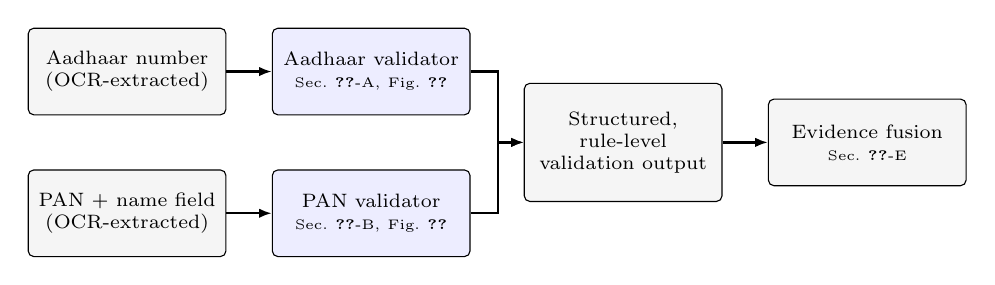
\begin{tikzpicture}[
  font=\scriptsize,
  box/.style={draw, rounded corners=2pt, align=center,
              minimum height=11mm, inner xsep=3pt, text width=23mm},
  src/.style={box, fill=black!4},
  val/.style={box, fill=blue!7},
  res/.style={box, fill=black!4, minimum height=15mm},
  ar/.style={-{Latex[length=1.6mm]}, thick}
]
\node[src] at (0,0.9)    (a-in)  {Aadhaar number\\(OCR-extracted)};
\node[src] at (0,-0.9)   (p-in)  {PAN $+$ name field\\(OCR-extracted)};
\node[val] at (3.1,0.9)  (a-val) {Aadhaar validator\\{\tiny Sec.~\ref{sec:framework}-A, Fig.~\ref{fig:aadhaar}}};
\node[val] at (3.1,-0.9) (p-val) {PAN validator\\{\tiny Sec.~\ref{sec:framework}-B, Fig.~\ref{fig:pan}}};
\node[res] at (6.3,0)    (out)   {Structured,\\rule-level\\validation output};
\node[box, fill=black!4, minimum height=11mm] at (9.4,0) (fuse)
     {Evidence fusion\\{\tiny Sec.~\ref{sec:method}-E}};
\draw[ar] (a-in) -- (a-val);
\draw[ar] (p-in) -- (p-val);
\draw[ar] (a-val.east) -- ++(0.35,0) |- (out.west);
\draw[ar] (p-val.east) -- ++(0.35,0) |- (out.west);
\draw[ar] (out) -- (fuse);
\end{tikzpicture}}
\caption{Overview of the structural/semantic validation framework.
Each validator independently produces a per-rule pass/fail/skip
result; Sections~\ref{sec:framework}-A and \ref{sec:framework}-B
specify the Aadhaar and PAN validators respectively,
Section~\ref{sec:framework}-C states the asymmetry between them, and
Section~\ref{sec:method}-E specifies how their outputs combine with
the visual branch.}
\label{fig:overview}
\end{figure}

\subsection{Aadhaar: Format and Verhoeff Checksum Validation}
\label{sec:aadhaar-validation}

An Aadhaar number is specified as a randomly generated eleven-digit
payload followed by a single Verhoeff check digit, giving a total
length of twelve decimal digits and a nominal payload space of
$10^{11}$~\cite{uidai-scheme}. A widely implemented convention
additionally holds that issued numbers do not begin with $0$ or $1$;
no authoritative statement of that restriction could be located in the
primary numbering document, so it is treated here as a convention
rather than as a specification. The validator specified below
accordingly does \emph{not} enforce it, checking length and checksum
only. The generator of Section~\ref{subsec:identifiers} does honour
it, which yields a smaller -- and therefore, for the coincidence
calculation given there, more conservative -- payload space of
$8 \times 10^{10}$.

Aadhaar validation applies two sequential checks. The format check
verifies that the extracted string $n = n_1 n_2 \dots n_{12}$ consists
of exactly 12 numeric digits; any deviation fails immediately and
short-circuits the checksum step, since a checksum is meaningful only
over a correctly-formatted sequence.

The checksum check implements the Verhoeff algorithm~\cite{verhoeff},
which detects all single-digit substitution errors and all
adjacent-digit transposition errors -- a stronger guarantee than a
simple modulus check. The algorithm is defined over a multiplication
table $D \in \mathbb{Z}^{10\times10}$ derived from the dihedral group
$D_5$ and a permutation table $P \in \mathbb{Z}^{8\times10}$ applied
cyclically by digit position. Table~\ref{tab:verhoeff} reproduces both
tables exactly as implemented, so that the checksum computation in
(\ref{eq:verhoeff}) is fully auditable. A third table, the inverse
table $\mathrm{inv}[\cdot]$, is required only when \emph{generating} a
check digit and plays no part in validation; it is used in this study
solely to construct the synthetic identifiers of
Section~\ref{sec:dataset} and is therefore not reproduced
here.\footnote{Generation and validation differ in one respect:
validation applies $P[i \bmod 8]$ over all twelve digits with $i = 0$
at the check digit, whereas generation applies $P[(i+1) \bmod 8]$ over
the eleven payload digits and returns $\mathrm{inv}[c]$.}

For digits indexed in reverse order ($i = 0$ at the rightmost digit),
the running checksum $c$ is defined by the recurrence
\begin{equation}
\label{eq:verhoeff}
\begin{split}
c_0     &= 0, \\
c_{i+1} &= D\big[\,c_i\,\big]\big[\,P[\,i \bmod 8\,][\,n_{12-i}\,]\,\big], \\
        &\qquad\qquad\qquad i = 0, 1, \dots, 11 .
\end{split}
\end{equation}

A number is structurally valid under this rule if and only if
$c_{12} = 0$. Algorithm~\ref{alg:aadhaar} gives the corresponding
procedure as implemented, using the same 1-indexed convention as
(\ref{eq:verhoeff}). Figure~\ref{fig:aadhaar} shows the full decision
flow.

\begin{table}[!tb]
\caption{Verhoeff Multiplication Table $D$ (top) and Permutation
Table $P$ (bottom)}
\label{tab:verhoeff}
\centering
\footnotesize
\setlength{\tabcolsep}{3.2pt}
\begin{tabular}{c|cccccccccc}
\toprule
$D$ & 0 & 1 & 2 & 3 & 4 & 5 & 6 & 7 & 8 & 9 \\
\midrule
0 & 0 & 1 & 2 & 3 & 4 & 5 & 6 & 7 & 8 & 9 \\
1 & 1 & 2 & 3 & 4 & 0 & 6 & 7 & 8 & 9 & 5 \\
2 & 2 & 3 & 4 & 0 & 1 & 7 & 8 & 9 & 5 & 6 \\
3 & 3 & 4 & 0 & 1 & 2 & 8 & 9 & 5 & 6 & 7 \\
4 & 4 & 0 & 1 & 2 & 3 & 9 & 5 & 6 & 7 & 8 \\
5 & 5 & 9 & 8 & 7 & 6 & 0 & 4 & 3 & 2 & 1 \\
6 & 6 & 5 & 9 & 8 & 7 & 1 & 0 & 4 & 3 & 2 \\
7 & 7 & 6 & 5 & 9 & 8 & 2 & 1 & 0 & 4 & 3 \\
8 & 8 & 7 & 6 & 5 & 9 & 3 & 2 & 1 & 0 & 4 \\
9 & 9 & 8 & 7 & 6 & 5 & 4 & 3 & 2 & 1 & 0 \\
\bottomrule
\end{tabular}

\vspace{5pt}

\begin{tabular}{c|cccccccccc}
\toprule
$P$ & 0 & 1 & 2 & 3 & 4 & 5 & 6 & 7 & 8 & 9 \\
\midrule
$i=0$ & 0 & 1 & 2 & 3 & 4 & 5 & 6 & 7 & 8 & 9 \\
$i=1$ & 1 & 5 & 7 & 6 & 2 & 8 & 3 & 0 & 9 & 4 \\
$i=2$ & 5 & 8 & 0 & 3 & 7 & 9 & 6 & 1 & 4 & 2 \\
$i=3$ & 8 & 9 & 1 & 6 & 0 & 4 & 3 & 5 & 2 & 7 \\
$i=4$ & 9 & 4 & 5 & 3 & 1 & 2 & 6 & 8 & 7 & 0 \\
$i=5$ & 4 & 2 & 8 & 6 & 5 & 7 & 3 & 9 & 0 & 1 \\
$i=6$ & 2 & 7 & 9 & 3 & 8 & 0 & 6 & 4 & 1 & 5 \\
$i=7$ & 7 & 0 & 4 & 6 & 9 & 1 & 3 & 2 & 5 & 8 \\
\bottomrule
\end{tabular}
\end{table}

\begin{algorithm}[!tb]
\caption{Aadhaar Verhoeff Checksum Validation}
\label{alg:aadhaar}
\begin{algorithmic}[1]
\Require 12-digit string $n = n_1 n_2 \dots n_{12}$; tables $D$, $P$
\Ensure \textsc{True} if $n$ is checksum-consistent, else \textsc{False}
\State $c \gets 0$
\For{$i \gets 0$ \textbf{to} $11$}
    \Comment{$i = 0$ selects $n_{12}$, the check digit}
    \State $c \gets D\big[\,c\,\big]\big[\,P[\,i \bmod 8\,][\,n_{12-i}\,]\,\big]$
\EndFor
\State \Return $(c = 0)$
\end{algorithmic}
\end{algorithm}

% ---------- FIGURE 2: Aadhaar validation flow ----------
\begin{figure}[!tb]
\centering
\resizebox{0.92\columnwidth}{!}{%
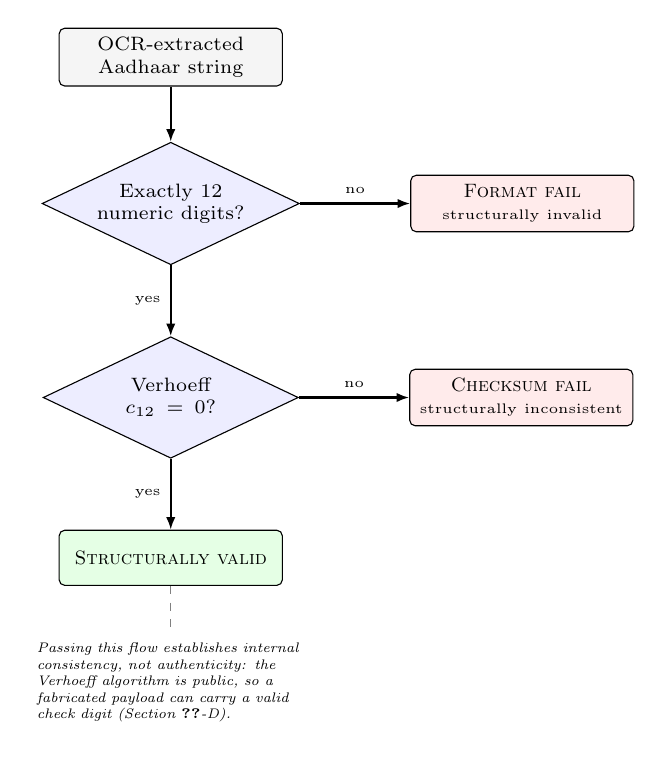
\begin{tikzpicture}[
  font=\scriptsize,
  node distance=7mm,
  io/.style={draw, rounded corners=2pt, align=center, fill=black!4,
             minimum height=7mm, text width=26mm},
  dec/.style={draw, diamond, aspect=2.1, align=center, fill=blue!7,
              inner sep=1pt, text width=20mm},
  fail/.style={draw, rounded corners=2pt, align=center, fill=red!8,
               minimum height=7mm, text width=26mm},
  ok/.style={draw, rounded corners=2pt, align=center, fill=green!10,
             minimum height=7mm, text width=26mm},
  note/.style={align=left, text width=34mm, font=\tiny\itshape},
  ar/.style={-{Latex[length=1.6mm]}, thick}
]
\node[io] (in) {OCR-extracted\\Aadhaar string};
\node[dec, below=of in] (d1) {Exactly 12\\numeric digits?};
\node[dec, below=9mm of d1] (d2) {Verhoeff\\$c_{12} = 0$?};
\node[ok, below=9mm of d2] (val) {\textsc{Structurally valid}};
\node[fail, right=14mm of d1] (f1)
     {\textsc{Format fail}\\{\tiny structurally invalid}};
\node[fail, right=14mm of d2] (f2)
     {\textsc{Checksum fail}\\{\tiny structurally inconsistent}};
\node[note, below=6mm of val.south, anchor=north] (n)
     {Passing this flow establishes internal consistency, not
      authenticity: the Verhoeff algorithm is public, so a fabricated
      payload can carry a valid check digit
      (Section~\ref{sec:framework}-D).};
\draw[ar] (in) -- (d1);
\draw[ar] (d1) -- node[left, font=\tiny] {yes} (d2);
\draw[ar] (d2) -- node[left, font=\tiny] {yes} (val);
\draw[ar] (d1) -- node[above, font=\tiny] {no} (f1);
\draw[ar] (d2) -- node[above, font=\tiny] {no} (f2);
\draw[dashed, gray] (val.south) -- (n.north);
\end{tikzpicture}}
\caption{Aadhaar structural validation flow: format check, then the
Verhoeff checksum of (\ref{eq:verhoeff}). The format check
short-circuits, since a checksum is meaningful only over a
correctly-formed 12-digit sequence.}
\label{fig:aadhaar}
\end{figure}

\subsection{PAN: Format, Category, and Cross-Field Semantic Rules}

PAN validation applies three checks -- two structural, one semantic --
reflecting the narrower validation capability available for this
document type (Section~\ref{sec:framework}-C). The format check
verifies the fixed pattern \texttt{AAAAA9999A} (five uppercase
letters, four digits, one uppercase letter).

The category check is structural: the fourth character $p_4$ is
matched against the fixed lookup in Table~\ref{tab:pancat}, as stated
in the Income Tax Department's PAN documentation~\cite{itd-pan}. A value of $p_4$
outside this set fails the check regardless of the remaining
structure.

\begin{table}[!tb]
\caption{PAN Taxpayer-Category Codes (Position 4)}
\label{tab:pancat}
\centering
\footnotesize
\begin{tabular}{cl}
\toprule
Code & Category \\
\midrule
P & Individual \\
C & Company \\
H & Hindu Undivided Family (HUF) \\
F & Firm \\
A & Association of Persons (AOP) \\
T & Trust \\
B & Body of Individuals (BOI) \\
L & Local Authority \\
J & Artificial Juridical Person \\
G & Government \\
\bottomrule
\end{tabular}
\end{table}

The name-consistency check is this study's semantic rule. The fifth
character $p_5$ encodes the first letter of the holder's surname for
Individual-category PANs ($p_4 = \texttt{P}$), and the first letter of
the entity's name for every non-Individual
category~\cite{itd-pan}. The check is therefore applicable to all
categories, with only the applicable name source differing; it is
scoped to Individual PANs in the difficult direction only, since for a
non-Individual holder the printed name is a single entity name whose
first character is unambiguous, whereas for an individual, evaluating
the rule against an OCR-extracted name field requires deciding
\emph{which} token of that field is the surname, and this is not a
trivial mapping in the Indian context.
Aadhaar and PAN print the holder's name as a single unlabelled line,
and Indian naming conventions are not uniform: many South Indian names
place the family or village name first and abbreviate it to an initial
(``V.\ Lakshmi''), some holders have no surname at all, and patronymic
and mononymic forms are both common. A rule that simply took the last
whitespace-delimited token as the surname would therefore report a
semantic failure on a substantial population of \emph{genuine}
documents, contaminating exactly the measurement this study is
designed to make.

This study consequently evaluates two variants of the rule and reports
both. Let $T = \textsc{Tokens}(\textit{name})$ be the alphabetic
tokens of the extracted name field after removing honorifics, with
single-letter abbreviated forms retained so that they contribute their
letter, and let $I = \{\, t_1 : t \in T \,\}$ be the set of token
initials. The \emph{permissive} rule, used as this study's primary
semantic check, is
\begin{equation}
\label{eq:sem}
\textit{sem}_{\text{perm}} =
\begin{cases}
(p_5 \in I)      & \text{if } p_4 = \texttt{P} \text{ and } T \neq \emptyset,\\[3pt]
(p_5 = T_{1,1})  & \text{if } p_4 \neq \texttt{P} \text{ and } T \neq \emptyset,\\[3pt]
\textsc{Skipped} & \text{if } T = \emptyset,
\end{cases}
\end{equation}
where $T_{1,1}$ denotes the first character of the first name token,
i.e.\ the entity-name rule for non-Individual categories.
and the \emph{strict} rule, reported alongside it as a sensitivity
analysis, replaces $I$ with the single initial of the final token,
$\{\,\textsc{Last}(T)_1\,\}$.

The permissive rule is the conservative choice: it fails only when
$p_5$ matches no initial present anywhere in the name field, which is
an unambiguous cross-field inconsistency under any naming convention,
at the cost of admitting forgeries in which a fabricated $p_5$ happens
to coincide with a non-surname initial. The strict rule is more
sensitive and correspondingly more brittle. Reporting the two together
separates the rule's detection capability from the naming convention
of the holder, and the gap between them is itself a reportable
quantity (Section~\ref{sec:results}). The dataset of
Section~\ref{sec:dataset} is stratified by naming convention --
surname-last, initial-first, and mononymic -- so that this gap is
measured rather than assumed. The case $T = \emptyset$, which arises
when OCR recovers no usable name field, is recorded as
\textsc{Skipped} rather than as a failure, since absence of evidence
is not inconsistency.

This remains a deterministic, rule-evaluable relationship between two
independently extracted fields, consistent with the narrow definition
of ``semantic'' given in Section~I-C, and involves no learned
inference. The remaining \textsc{Skipped} branch -- an empty token set
$T = \emptyset$, arising when OCR recovers no usable name field -- is
load-bearing: a validator that reported a failure when it had no name
to compare against would manufacture false positives out of extraction
failure. Absence of evidence is recorded as absence, not as
inconsistency.

Deliberately excluded from validation is the tenth character (check
digit), which the Income Tax Department documents as an alphabetic
check digit but for which no public specification of the generating
algorithm could be located~\cite{itd-pan}; it is therefore not
independently computable by any external system. The validator records
this as an inapplicable result rather than omitting it silently, so
that the rule-level explanation output
(Section~\ref{sec:method}-F) never implies a check digit was verified
when it was not. Algorithm~\ref{alg:pan} gives the full procedure and
Figure~\ref{fig:pan} the corresponding decision flow.

\begin{algorithm}[!tb]
\caption{PAN Structural and Semantic Validation}
\label{alg:pan}
\begin{algorithmic}[1]
\Require 10-character string $p = p_1 \dots p_{10}$; category table
         \textsc{Cat}; extracted name field \textit{name}
\Ensure  $(\textit{struct}, \textit{sem})$ with
         $\textit{struct} \in \{\textsc{True}, \textsc{False}\}$ and
         $\textit{sem} \in \{\textsc{True}, \textsc{False},
         \textsc{Skipped}\}$
\If{$p$ does not match \texttt{AAAAA9999A}}
    \State \Return $(\textsc{False}, \textsc{Skipped})$
    \Comment{format fail}
\EndIf
\If{$p_4 \notin \textsc{Cat}$}
    \State \Return $(\textsc{False}, \textsc{Skipped})$
    \Comment{category fail}
\EndIf
\State $T \gets \textsc{Tokens}(\textit{name})$
    \Comment{honorifics removed}
\If{$T = \emptyset$}
    \State \Return $(\textsc{True}, \textsc{Skipped})$
    \Comment{no usable name field}
\EndIf
\If{$p_4 = \texttt{`P'}$}
    \State $I \gets \{\, t_1 : t \in T \,\}$
        \Comment{individual: permissive, (\ref{eq:sem})}
    \State $\textit{sem}_{\text{strict}} \gets (p_5 = \textsc{Last}(T)_1)$
        \Comment{sensitivity analysis}
\Else
    \State $I \gets \{\, T_{1,1} \,\}$
        \Comment{entity name: first character}
\EndIf
\State $\textit{sem} \gets (p_5 \in I)$
\State \Return $(\textsc{True}, \textit{sem})$
\end{algorithmic}
\end{algorithm}

% ---------- FIGURE 3: PAN validation flow ----------
\begin{figure}[!tb]
\centering
\resizebox{0.96\columnwidth}{!}{%
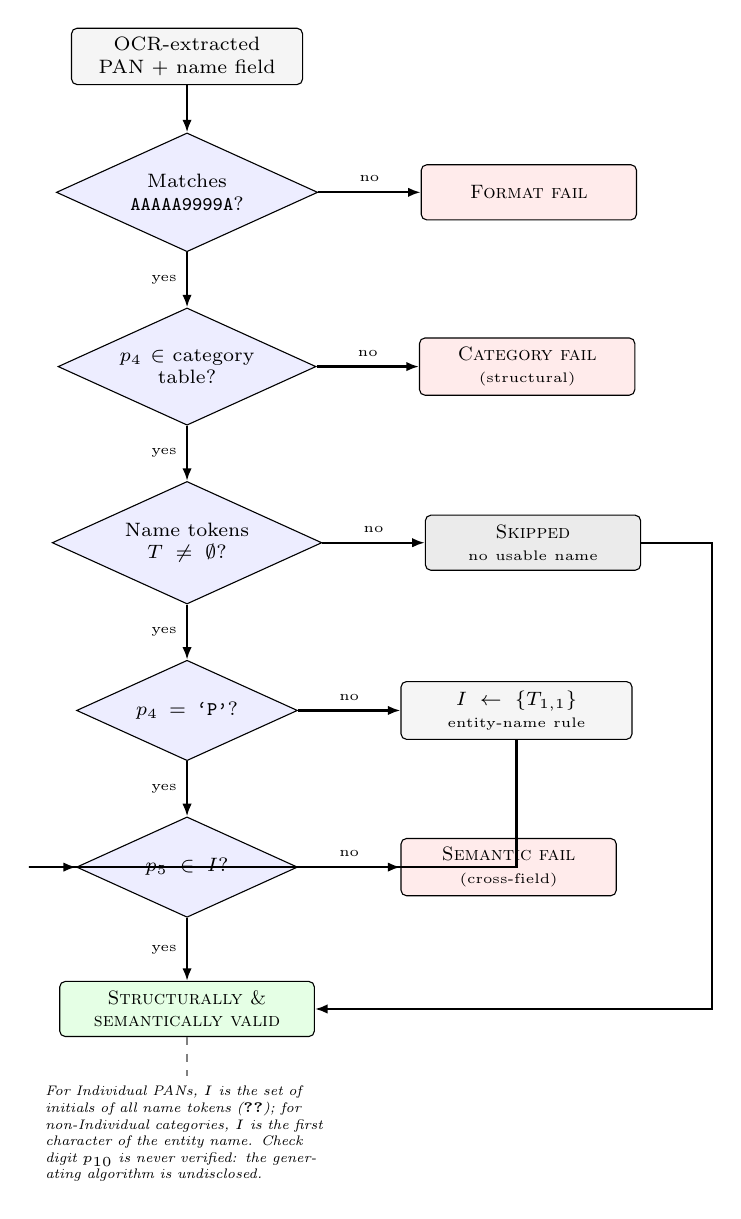
\begin{tikzpicture}[
  font=\scriptsize,
  node distance=6mm,
  io/.style={draw, rounded corners=2pt, align=center, fill=black!4,
             minimum height=7mm, text width=27mm},
  dec/.style={draw, diamond, aspect=2.2, align=center, fill=blue!7,
              inner sep=1pt, text width=21mm},
  fail/.style={draw, rounded corners=2pt, align=center, fill=red!8,
               minimum height=7mm, text width=25mm},
  skip/.style={draw, rounded corners=2pt, align=center, fill=black!8,
               minimum height=7mm, text width=25mm},
  ok/.style={draw, rounded corners=2pt, align=center, fill=green!10,
             minimum height=7mm, text width=30mm},
  ar/.style={-{Latex[length=1.6mm]}, thick}
]
\node[io] (in) {OCR-extracted\\PAN $+$ name field};
\node[dec, below=6mm of in]  (d1) {Matches\\\texttt{AAAAA9999A}?};
\node[dec, below=7mm of d1] (d2) {$p_4 \in$ category\\table?};
\node[dec, below=7mm of d2] (d3) {Name tokens\\$T \neq \emptyset$?};
\node[dec, below=7mm of d3] (d4) {$p_4 = \texttt{`P'}$?};
\node[dec, below=7mm of d4] (d5) {$p_5 \in I$?};
\node[ok,  below=8mm of d5] (val)
     {\textsc{Structurally \&}\\\textsc{semantically valid}};
\node[fail, right=13mm of d1] (f1) {\textsc{Format fail}};
\node[fail, right=13mm of d2] (f2) {\textsc{Category fail}\\{\tiny(structural)}};
\node[skip, right=13mm of d3] (s1) {\textsc{Skipped}\\{\tiny no usable name}};
\node[io,   right=13mm of d4] (s2) {$I \gets \{T_{1,1}\}$\\{\tiny entity-name rule}};
\node[fail, right=13mm of d5] (f3) {\textsc{Semantic fail}\\{\tiny(cross-field)}};
\node[align=left, text width=36mm, font=\tiny\itshape,
      below=5mm of val.south, anchor=north] (n)
     {For Individual PANs, $I$ is the set of initials of all name
      tokens (\ref{eq:sem}); for non-Individual categories, $I$ is the
      first character of the entity name. Check digit $p_{10}$ is
      never verified: the generating algorithm is undisclosed.};
\draw[ar] (in) -- (d1);
\draw[ar] (d1) -- node[left, font=\tiny] {yes} (d2);
\draw[ar] (d2) -- node[left, font=\tiny] {yes} (d3);
\draw[ar] (d3) -- node[left, font=\tiny] {yes} (d4);
\draw[ar] (d4) -- node[left, font=\tiny] {yes} (d5);
\draw[ar] (d5) -- node[left, font=\tiny] {yes} (val);
\draw[ar] (d1) -- node[above, font=\tiny] {no} (f1);
\draw[ar] (d2) -- node[above, font=\tiny] {no} (f2);
\draw[ar] (d3) -- node[above, font=\tiny] {no} (s1);
\draw[ar] (d4) -- node[above, font=\tiny] {no} (s2);
\draw[ar] (d5) -- node[above, font=\tiny] {no} (f3);
\draw[ar] (s1.east) -- ++(9mm,0) |- (val.east);
\draw[ar] (s2.south) |- ($(d5.west)+(-6mm,0)$) -- (d5.west);
\draw[dashed, gray] (val.south) -- (n.north);
\end{tikzpicture}}
\caption{PAN structural and semantic validation flow, per
(\ref{eq:sem}) and Table~\ref{tab:pancat}. The cross-field check
applies to every category; only the applicable name source differs.
The single \textsc{Skipped} branch -- an unrecoverable name field --
routes to the valid state rather than to a failure, since absence of
applicable evidence is not inconsistency.}
\label{fig:pan}
\end{figure}

\subsection{Scope and Asymmetry Between Aadhaar and PAN Validation}
\label{sec:asymmetry}

The two validators are deliberately asymmetric in what they check,
reflecting what each document format supports rather than an
implementation shortcut. Aadhaar's Verhoeff check digit is public and
independently computable, so its validator performs genuine
algorithmic verification: a failed checksum is a certain
inconsistency, not a heuristic signal. PAN's check digit algorithm is
not public, so no equivalent verification is possible for the tenth
character; PAN validation is instead limited to format, a fixed
category lookup, and one cross-field semantic rule.
Table~\ref{tab:capability} makes this asymmetry explicit rule by rule.
A ``fully valid'' result therefore carries different evidential weight
for the two document types, and the fusion strategy
(Section~\ref{sec:method}-E) is designed to preserve this distinction
rather than collapsing both into an undifferentiated ``passed
structural check'' signal. RQ5 tests whether this asymmetry produces a
measurable difference in incremental detection value.

\begin{table}[!tb]
\caption{Validation Capability: Aadhaar vs.\ PAN}
\label{tab:capability}
\centering
\footnotesize
\setlength{\tabcolsep}{4pt}
\begin{tabular}{p{2.3cm}p{1.9cm}p{2.7cm}}
\toprule
Rule & Aadhaar & PAN \\
\midrule
Format check & \checkmark & \checkmark \\
Category / type lookup & --- & \checkmark\ (structural) \\
Cross-field semantic check & --- & \checkmark\ (all categories; name source differs) \\
Independently verifiable check digit
  & \checkmark\ (Verhoeff, public)
  & $\times$ (undisclosed algorithm) \\
Guarantee on ``fully valid'' result
  & Certain algorithmic consistency
  & Format / category / semantic consistency only \\
\bottomrule
\end{tabular}
\end{table}

\subsection{Stated Limitations of Structural Validation}
\label{sec:limitations}

Two limitations bound what this framework can claim, both grounded in
implementation-level verification rather than asserted only in prose.

First, a failed check indicates internal inconsistency, not confirmed
forgery: the OCR layer (Section~\ref{sec:method}-C) can itself misread
a digit or character, producing a checksum or category failure on a
genuine document. This motivates the OCR-oracle comparison of
Section~\ref{sec:setup}-B (RQ4), which separates validator capability
from OCR-induced error.

Second, a passed check does not prove authenticity. Because the
Verhoeff algorithm is public, any fabricated eleven-digit payload can
be assigned a valid twelfth digit. The structural and semantic
validators are therefore correctly scoped as detectors of
unsophisticated, internally inconsistent forgery, not as authenticity
oracles.

Both validators were exercised against hand-constructed synthetic
inputs before integration. For Aadhaar these were a generated
checksum-consistent payload (\texttt{499785203517}), the same payload
with one interior digit altered (\texttt{499786203517}, correctly
rejected), a malformed non-12-digit input (rejected at the format
stage without the checksum being evaluated), and an independently
fabricated payload with its own correctly generated check digit
(\texttt{789456123005}), which is accepted -- the second limitation
above, exercised against running code, and the basis for the
structurally-valid-but-fabricated forgery category of
Section~\ref{sec:dataset}. For PAN they were an Individual-category
number with a consistent surname initial; the same number with $p_5$
altered, which is isolated to the semantic rule rather than the
format; an unrecognised $p_4$ category code; a Company-category number
whose $p_5$ matches the first character of the entity name, and the
same number with $p_5$ altered, exercising the non-Individual branch
of Algorithm~\ref{alg:pan} in both directions; a record with no
recoverable name field; and an initial-first name of the form
``V.~Lakshmi'' -- the last two routed through the \textsc{Skipped} and
permissive branches respectively, rather than failing. All identifiers
above are synthetic and correspond to no issued document.

\FloatBarrier
%======================================================================
\section{Dataset Construction}
\label{sec:dataset}

No public corpus pairs Aadhaar- or PAN-format document images with field-level
structural ground truth, so the incremental value this study measures cannot be
measured on existing data. MIDV-2020~\cite{midv}, IDNet~\cite{idnet} and
SIDTD~\cite{sidtd} establish that synthetic generation is the accepted substitute
for sensitive identity-document data, and this section follows that rationale
while adding what those corpora do not carry: for every image, the printed value
of every field, whether that value satisfies the rules of
Section~\ref{sec:framework}, and which field was corrupted to make it fail.

\subsection{Design Principles}
\label{subsec:principles}
\label{sec:ds-principles}

Four constraints govern the construction. Each is enforced by the generation
procedure rather than checked after the fact.

\emph{First, no real document is used at any stage.} All identifiers, names,
dates of birth, photographs and signatures are synthetic, following the privacy
rationale of SIDTD~\cite{sidtd} and MIDV-2020~\cite{midv}. No generated
identifier was submitted to, resolved through, or checked against any UIDAI or
Income Tax Department service, and no real identity-document image was
collected, downloaded or processed. Section~\ref{subsec:ethics} states what this
does and does not guarantee.

\emph{Second, the layouts are format-faithful and deliberately
design-unfaithful.} They reproduce the field structure of the two documents --
which fields are printed, in what order, with what identifier grouping -- because
that structure is what the validators of Section~\ref{sec:framework} operate on.
They do not reproduce any official emblem, seal, hologram, colour scheme or
authority name; a geometric placeholder mark and a fictitious authority name
stand in their place. Three layout variants exist per document type, differing
in typeface pairing, accent colour, label placement, photograph side and
background pattern density. Every rendered image carries an identical
low-opacity \textsc{synthetic specimen} overlay, composited before any forgery
operation and drawn identically for all categories, so that it cannot act as a
class-correlated cue. This choice costs realism and buys two things: the
released artefacts cannot function as documents, and the study is not obliged to
defend a pixel-level reproduction of a government design.

\emph{Third, the templates are authored rather than obtained.} Because no public
corpus supplies Aadhaar or PAN images with field-level structural ground truth,
both layouts were written as parameterised vector layouts and rasterised
directly. Exact field bounding boxes are therefore a by-product of rendering
rather than an annotation task, and they are propagated through the degradation
homography of Section~\ref{subsec:degrade} so that a field can be read from the
\emph{same pixels} both as ground truth and through OCR. That correspondence is
what makes the RQ4 comparison possible at all.

Figure~\ref{fig:pipeline} shows how the stages fit together and
Algorithm~\ref{alg:dataset} states the procedure as implemented.

\emph{Fourth, and most consequentially for the experimental claim, the forgery
categories intended to be visually undetectable are produced by re-rendering the
document from a modified identity record, not by editing a rendered image}, and
from the \emph{same render seed} as the genuine control, so that before
degradation the two images are identical outside the corrupted field. This is
developed in Section~\ref{subsec:taxonomy} and verified exactly in
Section~\ref{subsec:probe}.


\begin{figure*}[!t]
\centering
\resizebox{\textwidth}{!}{%
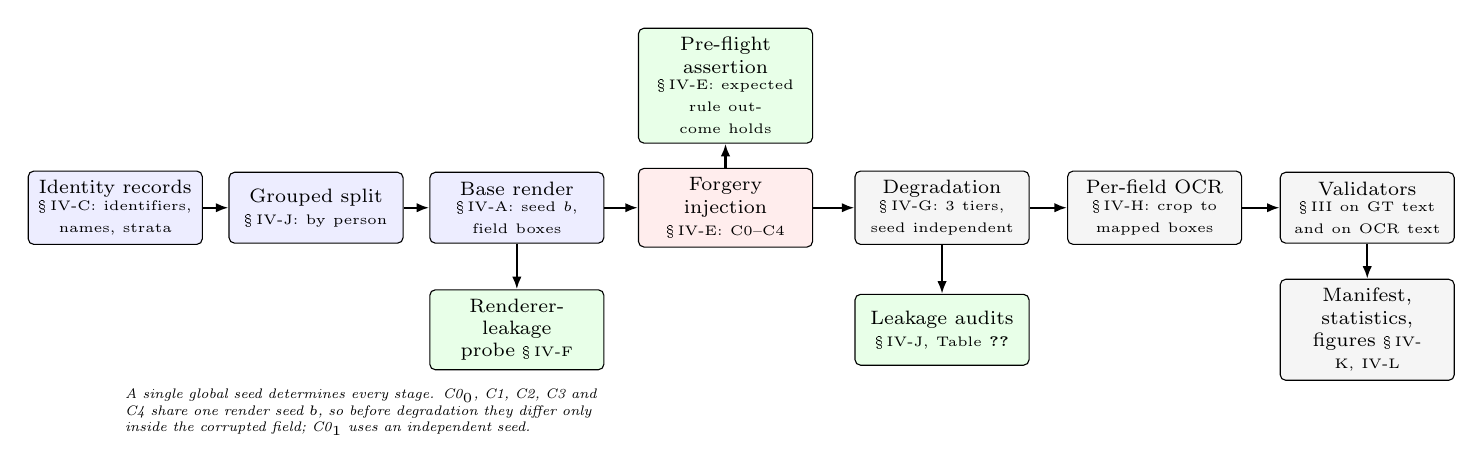
\begin{tikzpicture}[
  font=\scriptsize,
  box/.style={draw, rounded corners=2pt, align=center, minimum height=9mm,
              inner xsep=3pt, text width=20mm, fill=black!4},
  gen/.style={box, fill=blue!7},
  frg/.style={box, fill=red!7},
  aud/.style={box, fill=green!9},
  ar/.style={-{Latex[length=1.6mm]}, thick}
]
\node[gen] (rec)  at (0,0)    {Identity records\\{\tiny §\,IV-C: identifiers,\\names, strata}};
\node[gen] (spl)  at (2.55,0) {Grouped split\\{\tiny §\,IV-J: by person}};
\node[gen] (base) at (5.1,0)  {Base render\\{\tiny §\,IV-A: seed $b$,\\field boxes}};
\node[frg] (forg) at (7.75,0) {Forgery injection\\{\tiny §\,IV-E: C0--C4}};
\node[box] (deg)  at (10.5,0) {Degradation\\{\tiny §\,IV-G: 3 tiers,\\seed independent}};
\node[box] (ocr)  at (13.2,0) {Per-field OCR\\{\tiny §\,IV-H: crop to\\mapped boxes}};
\node[box] (val)  at (15.9,0) {Validators\\{\tiny §\,III on GT text\\and on OCR text}};
\node[aud] (pre)  at (7.75,1.55) {Pre-flight assertion\\{\tiny §\,IV-E: expected\\rule outcome holds}};
\node[aud] (prb)  at (5.1,-1.55) {Renderer-leakage\\probe {\tiny §\,IV-F}};
\node[aud] (lk)   at (10.5,-1.55) {Leakage audits\\{\tiny §\,IV-J, Table~\ref{tab:leakage}}};
\node[box] (man)  at (15.9,-1.55) {Manifest, statistics,\\figures {\tiny §\,IV-K, IV-L}};
\draw[ar] (rec) -- (spl);
\draw[ar] (spl) -- (base);
\draw[ar] (base) -- (forg);
\draw[ar] (forg) -- (deg);
\draw[ar] (deg) -- (ocr);
\draw[ar] (ocr) -- (val);
\draw[ar] (forg) -- (pre);
\draw[ar] (base) -- (prb);
\draw[ar] (deg) -- (lk);
\draw[ar] (val) -- (man);
\node[align=left, text width=62mm, font=\tiny\itshape, anchor=west]
  at (0,-2.6) {A single global seed determines every stage. C0$_0$, C1, C2, C3
  and C4 share one render seed $b$, so before degradation they differ only
  inside the corrupted field; C0$_1$ uses an independent seed.};
\end{tikzpicture}}
\caption{Dataset construction pipeline. Blue: generation. Red: the only stage
that introduces a forgery. Green: checks that gate the corpus rather than
describe it -- the pre-flight assertion (every category must produce its
expected rule outcome on ground-truth text), the renderer-leakage probe
(Section~\ref{subsec:probe}), and the five leakage audits
(Section~\ref{subsec:leakage}). A failure at any green node aborts the build;
none of them is reported as an experimental result.}
\label{fig:pipeline}
\end{figure*}

\begin{algorithm}[!t]
\caption{Corpus generation (single entry point)}
\label{alg:dataset}
\begin{algorithmic}[1]
\Require number of persons $N$; global seed $s$; template sets
\Ensure image corpus, manifest, splits, audits
\State $\mathcal{R} \gets \textsc{MakeRecords}(N, s)$
  \Comment{§\,\ref{subsec:records}}
\ForAll{$r \in \mathcal{R}$, document type $d$, category $c$}
  \State \textbf{assert} $\textsc{Rule}(d, \textsc{Fields}(r,d,c)) =
         \textsc{Expected}(d,c)$
  \Comment{pre-flight, §\,\ref{subsec:taxonomy}}
\EndFor
\State $\mathcal{S} \gets \textsc{GroupedStratifiedSplit}(\mathcal{R}, s)$
  \Comment{by person, §\,\ref{subsec:leakage}}
\ForAll{$r \in \mathcal{R}$, document type $d$}
  \State $b \gets \textsc{Seed}(s,r,d,\text{``base''})$;\;
         $a \gets \textsc{Seed}(s,r,d,\text{``alt''})$
  \State $(I_b, B) \gets \textsc{Render}(\textsc{Fields}(r,d), \text{tpl}(r,d), b)$
    \Comment{$B$: field boxes}
  \ForAll{$(c,i)$ in C0$_0$, C0$_1$, C1, C2, C3, C4}
    \If{$c = \text{C0} \wedge i = 1$}
      \State $I \gets \textsc{Render}(\textsc{Fields}(r,d),\text{tpl},a)$
    \ElsIf{$c = \text{C1}$}
      \State $I \gets \textsc{PixelEdit}(I_b, B)$
        \Comment{value-preserving}
    \Else
      \State $I \gets \textsc{Render}(\textsc{Modify}(\textsc{Fields}(r,d),c),
             \text{tpl}, b)$
        \Comment{same seed $b$}
    \EndIf
    \ForAll{tier $t \in \{\text{clean},\text{mild},\text{severe}\}$}
      \State $(J, B') \gets \textsc{Degrade}(I, t, \textsc{Seed}(s,r,d,c,i,t))$
      \State write $J$ to split $\mathcal{S}[r]$; record $B'$, seeds, provenance
    \EndFor
  \EndFor
\EndFor
\State $\textsc{Ocr}$ every field crop; run validators on ground-truth and on
       extracted text
\State run leakage audits, renderer-leakage probe, statistics, figures
\end{algorithmic}
\end{algorithm}

\subsection{Synthetic Identifier Generation}
\label{subsec:identifiers}
\label{sec:ds-identifiers}

Aadhaar identifiers are generated by sampling an eleven-digit payload and
appending the Verhoeff check digit computed with the same tables and code the
validator of Section~\ref{sec:framework}-A uses, so that a table transcription
error cannot produce a nominally genuine document that fails its own checksum.
PAN identifiers are generated by sampling three leading letters, a
taxpayer-category character $p_4$, a fifth character $p_5$ set from the
associated identity record as described in Section~\ref{subsec:records}, four
digits, and a final letter. The tenth character is sampled arbitrarily: because
its generating algorithm is undisclosed, this study neither validates nor
attempts to reproduce it, and the sampled letter must not be read as a check
digit.

The UIDAI numbering scheme specifies a twelve-digit number consisting of eleven
digits and one Verhoeff check digit, a nominal $10^{11}$ payload
space~\cite{uidai-scheme}. A widely implemented convention additionally holds that
issued numbers do not begin with $0$ or $1$; no authoritative UIDAI statement of
that restriction could be located, so it is treated here as a convention rather
than a specification. Generation honours it, giving a payload space of
$\dsAadhaarSpace$; validation does not enforce it, checking only length and
checksum as Section~\ref{sec:framework}-A specifies. Honouring it in generation
yields the smaller, and therefore more conservative, space for the calculation
that follows.

\paragraph*{Coincidence with issued identifiers} A synthetic identifier that is
format- and checksum-valid can, by arithmetic necessity, coincide with an
identifier that has actually been issued. This is not a defect that can be
engineered away; it follows from the density of the issued population within the
identifier space, and it applies to any synthetic corpus that generates
checksum-valid numbers. The corpus contains $\dsAadhaarStrings$ distinct
checksum-valid Aadhaar strings and $\dsPanStrings$ distinct PAN strings. Against
an issued Aadhaar population of order $1.4\times10^{9}$ within a space of
$\dsAadhaarSpace$, the per-identifier coincidence probability is approximately
$\dsAadhaarCoinPct\%$, giving an expectation of about $\dsAadhaarCoinExp$
coincidences. Under the constraints this generator applies -- three free
letters, one of ten category letters, one name-determined letter, four digits,
one free letter -- the effective PAN space is about $\dsPanSpace$; against an
issued population of order $8\times10^{8}$ the per-identifier probability is
$\dsPanCoinPct\%$ and the expectation about $\dsPanCoinExp$. In both cases the
probability that at least one generated identifier coincides with an issued one
is indistinguishable from unity.

It would therefore be false to describe such coincidence as negligible, and this
paper does not. The argument that the release is safe rests on \emph{non-linkage}
rather than on non-coincidence, and is stated in Section~\ref{subsec:ethics}.

\subsection{Identity Records and Naming Strata}
\label{subsec:records}
\label{sec:ds-identities}

Identity records are generated before documents, and every downstream artefact
inherits the same person identifier: both card types, all forgery categories and
all quality tiers derived from one record carry one \texttt{person\_id}. This is
what makes the grouped partition of Section~\ref{subsec:leakage} possible. Each
record carries a name in Latin and Devanagari script, a date of birth, a gender,
an Aadhaar number, a PAN, a procedurally drawn photograph and signature, and a
template-variant assignment per document type.

Names are drawn from a corpus of common Indian given names and surnames and
assigned to three naming strata in approximately equal proportion:
\emph{surname-last} (``Ananya Shukla''), \emph{initial-first} (``V. Lakshmi'')
and \emph{mononymic} (``Rajesh''). A fraction of records additionally carry a
printed honorific, exercising the honorific-stripping step of
$\textsc{tokens}(\cdot)$. This stratification exists to support the
permissive-versus-strict comparison of~(2): a corpus composed entirely of
surname-last names would make the two rule variants behave identically and would
misrepresent the false-positive behaviour of the cross-field rule on genuine
documents held by a large part of the population. Table~\ref{tab:permstrict}
shows that this is not a hypothetical concern.

For the initial-first stratum, which token the tax record treated as the surname
is genuinely ambiguous, so the generator draws $p_5$ either from the abbreviated
leading token or from the expanded given name. The prevalence of the former is a
\emph{modelling assumption}, not a measurement, and it is recorded per record as
\texttt{pan\_fifth\_source}. Every result conditioned on that field is
independent of the assumed prevalence; corpus-level rates are not, and are
reported as such.

\subsection{Dataset Composition}
\label{subsec:composition}
\label{sec:ds-composition}

The released corpus comprises $\dsPersons$ identity records, each contributing
one Aadhaar-format and one PAN-format record. Each record is rendered into six
documents -- two unmodified controls and one instance of each of the four
forgery categories -- and each document is captured at $\dsNq$ quality tiers,
giving $\dsDocuments$ documents and $\dsImages$ images, of which $\dsGenuine$
are genuine and $\dsForged$ forged. Every (document type $\times$ forgery
category) cell contains $\dsCellImages$ images, or $\dsCellControls$ for the
controls. Realised counts are given in Table~\ref{tab:forgery}. All detection
metrics in Section~\ref{sec:results} are reported with $95\%$ confidence
intervals, since the per-cell count is the binding constraint on what can be
claimed. At $\dsCellImages$ images per cell a proportion near $0.9$ is estimated
to about $\pm\dsCICell$ percentage points if images are treated as independent;
they are not, because the $\dsNq$ quality tiers of one document and the six
documents of one record share an identity, so the appropriate unit is the person
and the corresponding interval is about $\pm\dsCIPerson$ points. Interval
estimates in Section~\ref{sec:results} are clustered at the person level
accordingly.

Figure~\ref{fig:specimens} shows one record rendered across all five categories
in both formats, with the corrupted region marked;
Figure~\ref{fig:qualitytiers} shows one document across the three quality tiers;
Figure~\ref{fig:templates} shows the six layout variants. Each figure records in
the released artefacts the exact image identifiers it was drawn from, so any
panel can be traced back to a file in the corpus.

\begin{table*}[t]
\caption{Forgery categories, their intended
detectability, and the realised image counts per document type.
$\dsCellControls$ control images per document type comprise two
unmodified renders of every record at $\dsNq$ quality tiers. C2, C3
and C4 are produced by re-rendering from a modified record, so they
carry no pixel-level trace; C1 is the only category in which pixels
are edited after rendering, and it leaves every printed value valid.}
\label{tab:forgery}
\centering
\footnotesize
\begin{tabular}{@{}l p{7.2cm} l p{2.7cm} r r@{}}
\toprule
Cat. & Construction & Visual branch & Rule branch & Aadhaar & PAN \\
\midrule
C0 & Unmodified render & pass & pass & 1800 & 1800 \\
C1 & Post-render pixel edit; every printed value remains valid & detect & pass & 900 & 900 \\
C2 & Re-render with a structurally invalid identifier: Aadhaar checksum broken, or PAN format or category character broken & miss & detect & 900 & 900 \\
C3 & Re-render with a semantically inconsistent field pair: PAN fifth character against the name, Aadhaar Latin against Devanagari name & miss & detect (PAN only) & 900 & 900 \\
C4 & Re-render with a fabricated identifier that satisfies every rule & miss & miss & 900 & 900 \\
\bottomrule
\end{tabular}
\end{table*}


\begin{figure*}[t]
  \centering
  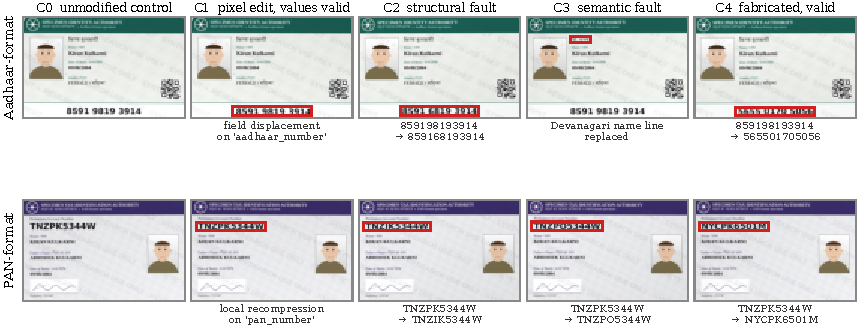
\includegraphics[width=\textwidth]{figures/fig_specimens.pdf}
  \caption{One synthetic identity record rendered across the five forgery
  categories, Aadhaar-format above and PAN-format below, at the clean quality
  tier. The corrupted region is boxed. C1 modifies pixels while leaving every
  printed value valid; C2, C3 and C4 modify a field value and are re-rendered,
  so they carry no pixel-level trace. All identifiers, names and photographs are
  synthetic; the emblem is a placeholder and the authority name is fictitious.}
  \label{fig:specimens}
\end{figure*}

\begin{figure*}[t]
  \centering
  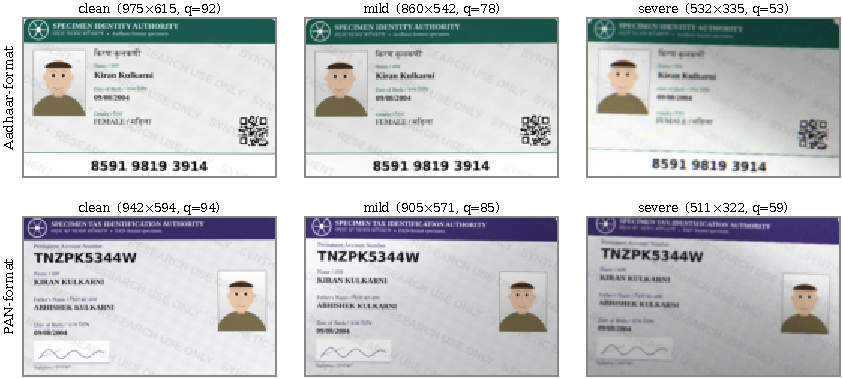
\includegraphics[width=\textwidth]{figures/fig_quality_tiers.pdf}
  \caption{The three capture quality tiers applied to one document, with output
  resolution and JPEG quality factor. Degradation is applied after forgery
  injection and drawn from an identical distribution for every forgery category.}
  \label{fig:qualitytiers}
\end{figure*}

\begin{figure*}[t]
  \centering
  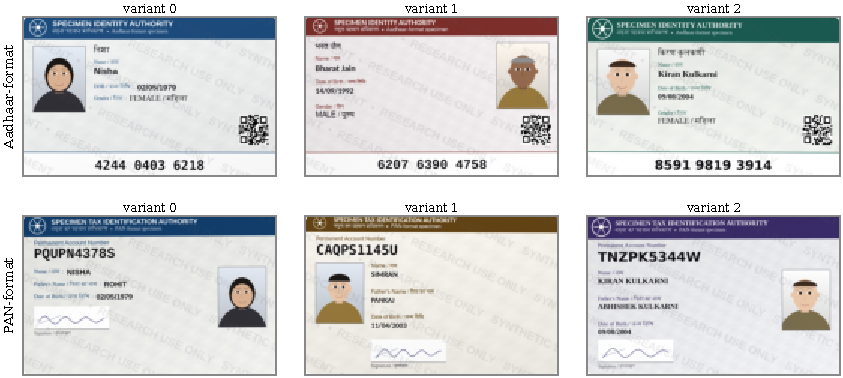
\includegraphics[width=\textwidth]{figures/fig_templates.pdf}
  \caption{The three layout variants per document type. Variants differ in
  typeface pairing, accent colour, label placement, photograph side and
  background pattern density; every variant is present in every split.}
  \label{fig:templates}
\end{figure*}

\subsection{Forgery Taxonomy}
\label{subsec:taxonomy}
\label{sec:ds-forgery}

Each base record is rendered into six documents: two unmodified controls and one
instance of each of the four forgery categories summarised in
Table~\ref{tab:forgery}.

\textbf{C1} is the only category in which pixels are modified after rendering.
It applies the standard document-tampering repertoire established by
DocTamper~\cite{doctamper} and CMID~\cite{cmid} -- copy-move patch splicing, small
field displacement, font substitution, localised recompression, and patch
resampling -- while leaving every printed value unchanged. The rule branch is
therefore expected to pass on C1, and only the visual branch has anything to
detect. The operation applied and the region affected are recorded per image,
giving localisation ground truth as a by-product.

\textbf{C2}, \textbf{C3} and \textbf{C4} are produced by modifying the identity
record and re-rendering the document through the same pipeline that produces the
controls. The resulting images share the fonts, antialiasing, guilloche phase
and compression history of a genuine render, so the only evidence distinguishing
them from a control is the content of the fields. Producing these categories by
pixel editing would introduce a visual artefact, allow the visual branch to
detect them through that artefact, and invalidate the incremental-value
measurement RQ2 and RQ3 are designed to make. This construction is therefore a
prerequisite of the experimental claim rather than an implementation
convenience.

\textbf{C4 is a deliberate negative control.} Both branches are expected to miss
it: the identifier is fabricated but carries a correctly generated check digit
and a consistent fifth character, so no implemented rule can object to it, and
the document is a genuine render, so no pixel-level trace exists. Reporting the
rate at which the branches do in fact fail on C4 converts the limitation stated
in Section~\ref{sec:framework}-D -- that a passed checksum does not prove
authenticity -- from an assertion into a measurement. One caveat must be carried
into the analysis: because the rule branch also fails on genuine documents
through OCR error (Section~\ref{subsec:characterisation}), a failure on C4 is an
OCR-induced false alarm and \emph{not} detection of the fabrication. Recall on
C4 is therefore not interpretable in isolation, and is reported alongside the
ground-truth-text verdict for the same image so the two causes can be separated.

\textbf{Aadhaar C3 is a deliberate asymmetry control.} Table~\ref{tab:capability} records that Aadhaar supports no cross-field
semantic rule. Omitting C3 from the Aadhaar arm would leave the two document
types with different category sets and would confound RQ5 with a difference in
dataset design. Instead the same \emph{class} of corruption is injected -- the
Latin and Devanagari renderings of the name, which on a genuine document name
the same person, are made to disagree -- and the Aadhaar validator is expected
to miss it, because no implemented rule reads the Devanagari line. RQ5 then
compares like with like: PAN detects this class of inconsistency and Aadhaar
does not, and the difference is attributable to validation capability rather
than to what was put in the dataset.

Before rendering at scale, every validator is run against the ground-truth text
of every generated document, requiring that C0 and C1 pass without exception,
that C2 fail without exception, that C3 fail without exception for PAN and pass
without exception for Aadhaar, and that C4 pass without exception. All
$\dsDocuments$ documents satisfy these conditions; the build aborts otherwise.
A deviation would indicate a generator defect and is not reported as an
experimental result. The complementary check -- that these categories are
visually indistinguishable from a control -- is the subject of
Section~\ref{subsec:probe}.


\subsection{Renderer-Leakage Probe}
\label{sec:dataset-probe}
\label{subsec:probe}

Everything RQ2 and RQ3 measure rests on one assumption: that C2, C3 and C4
documents carry \emph{no} visual evidence of forgery, because they are
re-rendered from a modified record and differ from a genuine control only in
the characters printed in one field. If the rendering pipeline leaked the label
-- through a different code path, a different rasterisation history, or a
layout that reflowed when a field value changed -- a visual detector could
separate those categories from C0 on a rendering artefact, the structural
branch's contribution would appear redundant, and the incremental-value
measurement would be measuring the artefact. The assumption is therefore tested
in two ways rather than asserted, and both tests are reported whatever their
outcome.

\paragraph*{Exact difference audit} C0$_0$, C1, C2, C3 and C4 are rendered from
a single shared render seed, so the guilloche phase, photograph, signature and
placeholder block are identical across them. Before degradation, a forged
document must therefore differ from its genuine control \emph{only} inside the
corrupted field's bounding box, or inside the edited region for C1. This is
checkable exactly rather than statistically: the audit re-renders every
category for \dsProbeRecords{} records, computes the pixel-wise difference
against the control, and counts the pixels that differ outside the expected
region. Over \dsProbeComparisons{} comparisons spanning \dsProbeCells{}
(document type $\times$ category) cells, that count is \textbf{\dsProbeOutside}.
The second control C0$_1$ is drawn with an independent seed, so the corpus is
not reduced to a single background per person.

This audit is not ceremonial. During development it detected a real defect: the
Aadhaar layout advanced each field by the measured extent of the text above it,
so a Devanagari name line of a different height shifted every field below it,
and the C3 script-mismatch category became visually separable through the
resulting reflow rather than through its intended semantic inconsistency. The
renderer was changed to use fixed vertical advances and the corpus regenerated.
A study that had asserted the assumption instead of testing it would have
reported the reflow as a visual-detection result.

\paragraph*{Learned probe} The exact audit governs the renders. The released
images are independently degraded and therefore do differ everywhere, so an
empirical check on them was also run: a gradient-boosted classifier over
downscaled pixels and low-frequency DCT coefficients, trained on the training
split to separate C0 from C2 $\cup$ C3 $\cup$ C4 and evaluated once on the test
split. Its balanced accuracy is \dsProbeCritical{} (95\% CI
\dsProbeCriticalCI, $n=\dsProbeCriticalN$).

That result is reported for completeness and should not be read as
confirmation. A probe too weak to learn anything returns $0.5$ as well, so the
same probe was run as a positive control on C0 versus C1, where a visual cue
exists by construction. It reaches only \dsProbeControl{}
(\dsProbeControlCI, $n=\dsProbeControlN$) over all tiers and
\dsProbeControlClean{} (\dsProbeControlCleanCI,
$n=\dsProbeControlCleanN$) on clean captures alone -- indistinguishable from
chance on a task that is known to be separable. The correct conclusion is that
this probe lacks the statistical power to certify anything, not that the
construction is confirmed: a downscaled-pixel model cannot resolve a font
substitution or a seven-pixel field displacement on a card reduced to fewer
than a hundred pixels on a side.

What carries the claim is therefore the exact difference audit, which is a
proof rather than a statistical test, together with the observation that the
degradation parameters are drawn from a distribution that depends only on the
quality tier and never on the forgery category. A properly powered version of
the probe -- the ResNet-50 branch of Section~\ref{sec:method}-B rather than a
gradient-boosted model over thumbnails -- is reported in
Section~\ref{sec:results}. The construction predicts near-chance performance
there as well, and unlike the probe reported here that prediction will be
falsifiable.

\subsection{Image Quality and Degradation}
\label{subsec:degrade}
\label{sec:ds-quality}

Clean renders yield near-perfect OCR and would collapse RQ4 into a degenerate
comparison. Each document is therefore captured at three quality tiers --
\emph{clean}, \emph{mild}, \emph{severe} -- through a seeded capture simulation
implemented directly on NumPy and OpenCV: a single composed homography
(perspective, rotation, scale), an illumination gradient, an optional cast
shadow, optical and occasional motion blur, a moir\'e interference term, sensor
noise, chromatic shift, and JPEG compression at a tier-dependent quality factor.
The released file is the compressed byte stream produced by that last stage, not
a re-encoding of it, so no artificial second compression is layered on top of the
simulated capture. General-purpose document-degradation libraries such as
Augraphy~\cite{augraphy} implement a comparable chain; the pipeline is written here
instead so that the corpus reproduces from the repository with no dependency
beyond NumPy, OpenCV and Pillow, and so that every applied parameter is recorded
per image in the manifest.

Degradation is applied \emph{after} forgery injection, so a C1 pixel edit is
subject to the same degradation as the surrounding document and cannot be
identified by the absence of capture artefacts. The tier is drawn from an
identical distribution for every forgery category, so image quality cannot act
as a class cue. The per-image seed, output resolution and quality factor are
recorded in the manifest.

\subsection{OCR Extraction}
\label{subsec:ocr}
\label{sec:ds-ocr}

Field values are extracted by cropping to the ground-truth bounding boxes mapped
through the degradation homography and applying Tesseract~\cite{tesseract} per field
with a character whitelist appropriate to the field type. Raw output is stored
without correction. A minimal and explicitly documented \emph{parsing} step is
applied before the validators see a string -- whitespace removal for the two
identifier fields, which are printed in groups, and whitespace normalisation for
name fields -- and nothing else. No character substitution, dictionary lookup,
checksum-guided repair or confidence-based rejection is applied, because the gap
between validator behaviour on ground-truth text and on extracted text
\emph{is} the RQ4 measurement, and repairing the output would destroy it.

The whitelists are flat over the field's character class rather than
position-aware. A position-aware whitelist for PAN -- letters at positions 1--5
and 10, digits at 6--9 -- would eliminate most of the confusions reported in
Section~\ref{subsec:characterisation} and would drive the format check's
false-positive rate towards zero. It would do so by constraining the extractor
with exactly the format the validator then checks, making the format check
partly self-fulfilling and inflating the apparent quality of the structural
branch. The flat whitelist is the conservative choice and is the one used.

Two limitations follow from the available OCR model. Only the English Tesseract
model is used, so the Devanagari name line is rendered but not extracted; the
Aadhaar C3 corruption is consequently unreadable by the pipeline by
construction, which is the intended negative control but also means the Aadhaar
semantic gap is demonstrated rather than closed. Second, a robustness check
against an independent second engine is not performed here; the extraction
interface accepts an alternative engine and this is left to
Section~\ref{sec:discussion-threats} as a stated threat rather than claimed as done.

\subsection{Corpus Characterisation and Validator Behaviour}
\label{subsec:characterisation}

The measurements in this subsection characterise the \emph{corpus} and the rule
branch operating on it. No visual model is trained and no fusion is performed at
this stage, so none of these numbers is a detection result for the hybrid
system; they are the inputs on which Sections~\ref{sec:setup}
and~\ref{sec:results} build, and they establish that the corpus has the
properties the experimental design assumes.

Table~\ref{tab:ocr} and Figure~\ref{fig:ocr} report per-field extraction
quality. The Aadhaar number is recovered exactly on
$\dsOcrAadhaarAadhaarNumberClean\%$ of clean captures and
$\dsOcrAadhaarAadhaarNumberSevere\%$ of severe ones. The PAN number is recovered
on only $\dsOcrPanPanNumberClean\%$ of clean captures, falling to
$\dsOcrPanPanNumberSevere\%$ under severe degradation. The gap between the two
identifier fields at the same capture quality is instructive and is not a
degradation effect: a PAN mixes letters and digits without positional
constraint at the extractor, and the dominant residual errors are the
character-shape confusions $0\!\leftrightarrow\!\mathrm{O}$,
$\mathrm{I}\!\leftrightarrow\!1$ and $5\!\rightarrow\!\mathrm{S}$, together with
occasional insertions that change the string length. An Aadhaar number, being
purely numeric, admits no such confusion.

Table~\ref{tab:rulerate} reports the rule-branch flag rate by category on
ground-truth text and on extracted text. On ground-truth text the branch behaves
exactly as designed: it flags $100\%$ of C2 for both document types and $100\%$
of PAN C3, and $0\%$ of everything else. On extracted text this structure
survives -- C2 and PAN C3 remain near-saturated -- but a floor of spurious
failures appears in every other cell, and that floor is the cost of operating on
real OCR output.

Table~\ref{tab:fpr} isolates that cost on genuine documents, which is the
measurement RQ6 requires. On ground-truth text the false-positive rate is zero
by construction, so every entry is attributable to extraction error. For Aadhaar
it rises from $\dsFPAadhaarClean\%$ on clean captures to
$\dsFPAadhaarSevere\%$ on severe ones. For PAN it is $\dsFPPanClean\%$ even on
clean captures and $\dsFPPanSevere\%$ on severe ones -- an order of magnitude
above Aadhaar at the same capture quality. The asymmetry that
Section~\ref{sec:asymmetry} treats as an advantage for PAN, namely that PAN
supports more independent checks than Aadhaar, is therefore also a liability:
more rules applied to a harder-to-extract field produce more opportunities to
fail on a genuine document. Any fusion rule that treats a structural failure as
evidence of forgery inherits this rate, which is why RQ6 is included in the
question set and why a detection-only evaluation of the hybrid system would not
be interpretable.

Table~\ref{tab:permstrict} separates the permissive rule of~(2) from its strict
variant on genuine PAN documents. On ground-truth text the permissive rule never
fails, as it must not. The strict variant fails on $\dsStrictAll\%$ of all genuine
documents, and that failure is not spread evenly: it is confined entirely to the
initial-first stratum, where it reaches $\dsStrictInitialFirst\%$, and within
that stratum to records whose fifth character derives from the abbreviated
leading token, where it reaches $\dsStrictLeadingInitial\%$. The corpus-level figure depends on the modelling assumption
of Section~\ref{subsec:records} and should be read as conditional on it; the
stratified figures do not. This is the quantity Section~\ref{sec:framework}-B
identified as reportable, and it is the empirical justification for adopting the
permissive rule as this study's primary check: a rule that simply took the last
whitespace-delimited token as the surname would report a semantic failure for
close to one genuine document in three within a naming convention held by a
large population, contaminating exactly the measurement this study is designed
to make.

\begin{table}[t]
\caption{Per-field OCR extraction quality by capture quality tier:
exact-match rate with a 95\% Wilson interval, and mean character
error rate. Raw Tesseract output, with only the parsing step of
Section~\ref{subsec:ocr} applied.}
\label{tab:ocr}
\centering
\footnotesize
\begin{tabular}{@{}llrrr@{}}
\toprule
Field & Tier & $n$ & Exact match \% [95\% CI] & CER \% \\
\midrule
A: number & clean & 1800 & 99.8 [99.5, 99.9] & 0.01 \\
 & mild & 1800 & 99.4 [99.0, 99.7] & 0.07 \\
 & severe & 1800 & 88.3 [86.8, 89.7] & 2.50 \\
\addlinespace[1.5pt]
A: name & clean & 1800 & 98.8 [98.2, 99.2] & 0.10 \\
 & mild & 1800 & 98.7 [98.1, 99.2] & 0.10 \\
 & severe & 1800 & 64.7 [62.5, 66.9] & 22.22 \\
\addlinespace[1.5pt]
A: DOB & clean & 1800 & 100.0 [99.8, 100.0] & 0.00 \\
 & mild & 1800 & 100.0 [99.8, 100.0] & 0.00 \\
 & severe & 1800 & 41.5 [39.2, 43.8] & 45.33 \\
\addlinespace[1.5pt]
P: number & clean & 1800 & 85.2 [83.5, 86.7] & 1.57 \\
 & mild & 1800 & 84.9 [83.2, 86.5] & 1.57 \\
 & severe & 1800 & 67.7 [65.5, 69.8] & 7.30 \\
\addlinespace[1.5pt]
P: name & clean & 1800 & 99.7 [99.3, 99.8] & 0.04 \\
 & mild & 1800 & 99.6 [99.2, 99.8] & 0.06 \\
 & severe & 1800 & 53.8 [51.5, 56.1] & 31.78 \\
\addlinespace[1.5pt]
P: father & clean & 1800 & 100.0 [99.8, 100.0] & 0.00 \\
 & mild & 1800 & 100.0 [99.8, 100.0] & 0.00 \\
 & severe & 1800 & 44.7 [42.4, 47.0] & 43.68 \\
\addlinespace[1.5pt]
P: DOB & clean & 1800 & 99.7 [99.3, 99.9] & 0.03 \\
 & mild & 1800 & 99.9 [99.7, 100.0] & 0.01 \\
 & severe & 1800 & 33.8 [31.7, 36.0] & 50.84 \\
\bottomrule
\end{tabular}
\end{table}

\begin{table}[t]
\caption{Rule-branch flag rate by forgery category (\% of images on
which an applicable rule evaluated \textsc{false}), on ground-truth
text and on OCR-extracted text, with 95\% Wilson intervals. On C0 a
flag is a false positive. On C4 both branches are expected to miss by
construction, so a flag there is an OCR-induced false alarm and not
detection of the fabrication.}
\label{tab:rulerate}
\centering
\footnotesize
\begin{tabular}{@{}llll@{}}
\toprule
Document & Cat. & Ground-truth text & OCR text \\
\midrule
Aadhaar & C0 & 0.0 [0.0, 0.2] & 4.1 [3.3, 5.1] \\
 & C1 & 0.0 [0.0, 0.4] & 4.1 [3.0, 5.6] \\
 & C2 & 100.0 [99.6, 100.0] & 99.8 [99.2, 99.9] \\
 & C3 & 0.0 [0.0, 0.4] & 3.9 [2.8, 5.4] \\
 & C4 & 0.0 [0.0, 0.4] & 4.0 [2.9, 5.5] \\
\midrule
PAN & C0 & 0.0 [0.0, 0.2] & 18.9 [17.1, 20.8] \\
 & C1 & 0.0 [0.0, 0.4] & 20.8 [18.3, 23.5] \\
 & C2 & 100.0 [99.6, 100.0] & 97.1 [95.8, 98.0] \\
 & C3 & 100.0 [99.6, 100.0] & 96.2 [94.8, 97.3] \\
 & C4 & 0.0 [0.0, 0.4] & 23.2 [20.6, 26.1] \\
\bottomrule
\end{tabular}
\end{table}

\begin{table}[t]
\caption{Rule-branch false-positive rate on \emph{genuine} documents
(category C0) as a function of capture quality, evaluated on
OCR-extracted text. On ground-truth text the rate is zero by
construction, so every entry here is attributable to OCR extraction
error. This is the measurement RQ6 requires.}
\label{tab:fpr}
\centering
\footnotesize
\begin{tabular}{@{}llrrl@{}}
\toprule
Document & Tier & $n$ & FP & FP rate \% [95\% CI] \\
\midrule
Aadhaar & clean & 600 & 2 & 0.3 [0.1, 1.2] \\
 & mild & 600 & 2 & 0.3 [0.1, 1.2] \\
 & severe & 600 & 70 & 11.7 [9.3, 14.5] \\
 & all & 1800 & 74 & 4.1 [3.3, 5.1] \\
\midrule
PAN & clean & 600 & 76 & 12.7 [10.2, 15.6] \\
 & mild & 600 & 73 & 12.2 [9.8, 15.0] \\
 & severe & 600 & 191 & 31.8 [28.2, 35.7] \\
 & all & 1800 & 340 & 18.9 [17.1, 20.8] \\
\bottomrule
\end{tabular}
\end{table}

\begin{table}[t]
\caption{PAN cross-field rule on \emph{genuine} documents:
permissive rule (2) against the strict variant, by naming stratum and
by the source of the fifth character. A failure here is a false
positive on a genuine document. The strict variant is reported as a
sensitivity analysis, not as the study's rule.}
\label{tab:permstrict}
\centering
\scriptsize
\setlength{\tabcolsep}{3.5pt}
\begin{tabular}{@{}llrll@{}}
\toprule
Subset & Text & $n$ & Permissive FAIL \% & Strict FAIL \% \\
\midrule
all genuine PAN & gt & 1800 & 0.0 [0.0, 0.2] & 9.0 [7.8, 10.4] \\
 & ocr & 1800 & 1.9 [1.4, 2.6] & 9.4 [8.2, 10.9] \\
\addlinespace[1.5pt]
surname-last & gt & 648 & 0.0 [0.0, 0.6] & 0.0 [0.0, 0.6] \\
 & ocr & 648 & 1.1 [0.5, 2.2] & 1.4 [0.7, 2.6] \\
\addlinespace[1.5pt]
initial-first & gt & 552 & 0.0 [0.0, 0.7] & 29.3 [25.7, 33.3] \\
 & ocr & 552 & 3.8 [2.5, 5.7] & 27.4 [23.8, 31.2] \\
\addlinespace[1.5pt]
mononymic & gt & 600 & 0.0 [0.0, 0.6] & 0.0 [0.0, 0.6] \\
 & ocr & 600 & 1.0 [0.5, 2.2] & 1.7 [0.9, 3.0] \\
\addlinespace[1.5pt]
$p_5$ from initial & gt & 174 & 0.0 [0.0, 2.2] & 93.1 [88.3, 96.0] \\
 & ocr & 174 & 6.9 [4.0, 11.7] & 81.0 [74.6, 86.2] \\
\addlinespace[1.5pt]
$p_5$ from given name & gt & 378 & 0.0 [0.0, 1.0] & 0.0 [0.0, 1.0] \\
 & ocr & 378 & 2.4 [1.3, 4.5] & 2.6 [1.4, 4.8] \\
\addlinespace[1.5pt]
\bottomrule
\end{tabular}
\end{table}


\begin{figure}[t]
  \centering
  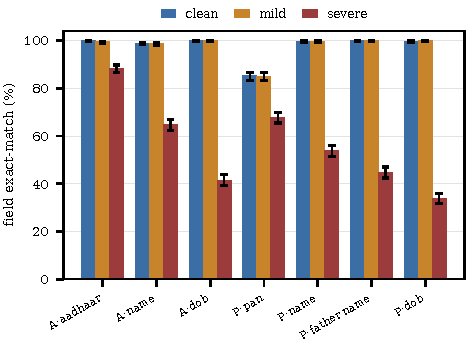
\includegraphics[width=\columnwidth]{figures/fig_ocr_quality.pdf}
  \caption{Per-field OCR exact-match rate by capture quality tier, with $95\%$
  Wilson intervals. ``A'' denotes Aadhaar-format fields and ``P'' PAN-format
  fields.}
  \label{fig:ocr}
\end{figure}

\subsection{Train/Validation/Test Split and Leakage Control}
\label{subsec:leakage}
\label{sec:ds-split}

Splits are made at the level of the person identifier, not the image and not the
document, and stratified over the naming stratum and both template-variant
assignments. An image-level split would place one identity's genuine and forged
documents on opposite sides of the partition, allowing a model to recognise the
identity rather than the forgery. Allocation uses a running largest-deficit rule
rather than per-stratum integer flooring, which at this number of strata would
systematically starve the two minority splits; the realised partition is
$\dsTrainPer/\dsValPer/\dsTestPer$ persons and
$\dsTrainImg/\dsValImg/\dsTestImg$ images. Fusion thresholds
(Section~\ref{sec:method}-E) are calibrated on the validation split only; the
test split is evaluated once.

Five leakage modes are audited on the released splits and the audit is reported
in Table~\ref{tab:leakage} rather than asserted. Four are exact and all pass: no
person identifier, no Aadhaar or PAN string, and no set of printed field values
occurs in more than one split, and no document's degradation draws span splits.

The fifth, near-duplicate detection by perceptual hashing, is reported as a
\emph{diagnostic rather than a gate}, because running it establishes that it
cannot serve as one here. Every document in this corpus shares one of six card
layouts, which dominates the low-frequency DCT band a perceptual hash is built
from. A $64$-bit hash is degenerate on this corpus: it yields only
$\dsPhashDistinctSixtyFour$ distinct values for $\dsImages$ images and collides
across different persons, different forgery categories and different splits. A
$\dsPhashBits$-bit hash separates images ($\dsPhashDistinct$ distinct values) but
still does not cleanly separate identities: the median distance between two
captures of the same document is $\dsPhashWithinMed$ bits and between two
different persons' documents $\dsPhashCrossPersonMed$ bits, but the
distributions overlap, with separability AUC $\dsPhashAUC$ and
$\dsPhashOverlap\%$ of different-person pairs closer than the median
same-document pair. No distance threshold can therefore distinguish a leaked
duplicate from two unrelated documents on the same template, and the smallest
cross-split distances are additionally a minimum taken over every training
image, which is small for that reason alone. Because the exact identity audit
already establishes that the splits are person-disjoint, every cross-split
neighbour is necessarily a different person, and these distances carry no
leakage information beyond what that audit establishes.
Figure~\ref{fig:phash} shows the three distance distributions. Reporting this
negatively is preferable to reporting a threshold-based pass that the measure
does not support.

\begin{table}[t]
\caption{Leakage audit performed on the released splits. Each check is
run on the corpus and its outcome reported, rather than asserted. The
first four checks are exact and all pass. The fifth, near-duplicate
detection by perceptual hashing, is reported as a \emph{diagnostic}
rather than a gate: on a corpus in which every document shares one
of six layout templates, the same-document and different-person
distance distributions overlap, so no threshold can separate a
leaked duplicate from two unrelated documents. See
Section~\ref{subsec:leakage} and Fig.~\ref{fig:phash}.}
\label{tab:leakage}
\centering
\scriptsize
\setlength{\tabcolsep}{3.5pt}
\begin{tabular}{@{}p{1.15cm}p{3.0cm}ll@{}}
\toprule
Leakage mode & Check & Required & Observed \\
\midrule
Identity & person-id intersection across splits & empty & 0 \\
Identifier & Aadhaar/PAN string intersection & empty & 0 \\
Template & every layout variant in every split & all & 6/6 \\
Near-duplicate & \dsPhashBits-bit perceptual-hash distance & (diagnostic) & see Sec.~\ref{subsec:leakage} \\
Augment\-ation & degradation draws of one document & one split & 0 span splits \\
Printed values & identical field-value set in two splits & none & 0 of 2100 \\
\bottomrule
\end{tabular}
\end{table}


\begin{figure}[t]
  \centering
  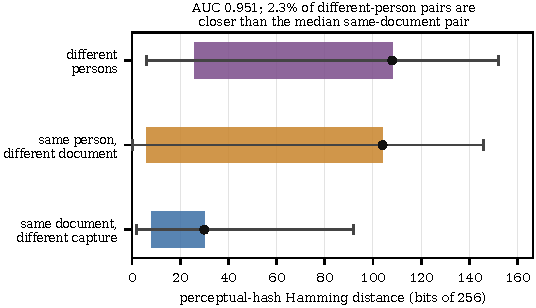
\includegraphics[width=\columnwidth]{figures/fig_phash_leakage.pdf}
  \caption{Perceptual-hash distance distributions ($\dsPhashBits$-bit hash);
  bars span the first percentile to the median, whiskers the full range, dots
  the median. The same-document and different-person distributions overlap, so
  the near-duplicate check is reported as a diagnostic and the leakage verdict
  rests on the exact audits of Table~\ref{tab:leakage}.}
  \label{fig:phash}
\end{figure}


\subsection{Reproducibility and Release}
\label{subsec:release}
\label{sec:ds-repro}

The dataset is reproducible from code. A single entry point regenerates
templates, identifiers, renders, forgeries, degradations, OCR output, splits,
audits and figures from one global seed, with dependency versions pinned, the
font binaries committed to the repository so that rasterisation does not depend
on the host system's installed faces, and the OCR binary version recorded. The
number of worker processes does not affect the output, because every random draw
is seeded from the person identifier rather than from execution order. Build
time is approximately $17$ minutes on two cores and the corpus occupies
$\dsGiB$\,GiB.

The release comprises the generation code, the configuration, the manifest and
the figures, from which the image corpus can be regenerated exactly; the built
corpus is additionally archived. The manifest records, per image: the image,
document and person identifiers; document type, forgery category, quality tier,
naming stratum, template variant and split; ground-truth and extracted field
values with per-field exact-match and character error rate; field bounding boxes
in the degraded image's coordinate frame; the corrupted field with its values
before and after; the C1 operation and its region; the render and degradation
seeds; and the validator output on both ground-truth and extracted text.

\subsection{Ethical Considerations}
\label{subsec:ethics}
\label{sec:ds-ethics}

No real Aadhaar or PAN document, image or number was collected, downloaded,
purchased or processed at any stage. All identifiers are synthetic. No
identifier was submitted to or verified against any government or third-party
identity service. No official emblem is reproduced; a visually distinct
placeholder mark is used in its place, the issuing authority named on the cards
is fictitious, and every image carries a permanent synthetic-specimen overlay.

As Section~\ref{subsec:identifiers} establishes quantitatively, a small
proportion of the generated identifiers can be expected to coincide with issued
ones, and it would be false to claim otherwise. The case that the release is
nonetheless safe rests on non-linkage rather than on non-coincidence. A bare
identifier string carrying no association to a real person is not information
about an identifiable person; in this corpus every identifier is printed
alongside a generated name, a generated date of birth and a procedurally drawn
placeholder, none of which belongs to any human being, so a coincident number
appears in the dataset attached to a person who does not exist. No identifier was
ever resolved or verified, so the corpus contains no information about whether
any string is issued and none about any holder. The expected coincidence count
is reported rather than suppressed, so a user of the dataset can reason about it
directly.

The released artefacts are intended to support evaluation of forgery
\emph{detection} and are not sufficient to produce a document capable of passing
any operational verification process, since structural validity is explicitly
shown in this study -- by category C4 -- not to establish authenticity.

\FloatBarrier
\section{Methodology}
\label{sec:method}

\subsection{System Overview and Pipeline}
\todosec{}

\subsection{Visual Detection Branch}
\todosec{}

\subsection{OCR and Field Extraction}
\todosec{Tesseract-based extraction~\cite{tesseract}.}

\subsection{Structural/Semantic Validation Branch}
\todosec{Implements Section~\ref{sec:framework} as specified.}

\subsection{Evidence Fusion Strategy}
\todosec{Must preserve the Aadhaar/PAN evidential asymmetry of
Table~\ref{tab:capability} rather than collapsing both into a single
``passed structural check'' signal.}

\subsection{Rule-Level Explanation Generation}
\todosec{Must never imply that the PAN check digit was verified.}

%======================================================================
\section{Experimental Setup}
\label{sec:setup}

\subsection{Configurations Compared}
\todosec{Visual-only, structural/semantic-only, and hybrid.}

\subsection{OCR Oracle Experiment}
\todosec{Ground-truth field values versus OCR-extracted values,
addressing RQ4.}

\subsection{Evaluation Metrics}
\todosec{}

\subsection{Implementation Details}
\todosec{}

%======================================================================
\section{Results}
\label{sec:results}

\subsection{RQ1: Visual Detector on Conventional Forgeries}
\todosec{}

\subsection{RQ2: Structural/Semantic Detector on Visually Plausible
Forgeries}
\todosec{}

\subsection{RQ3: Hybrid vs.\ Individual Evidence Sources by Forgery
Category}
\todosec{}

\subsection{RQ4: OCR Oracle -- Ground Truth vs.\ Actual OCR}
\todosec{}

\subsection{RQ5: Aadhaar vs.\ PAN Breakdown}
\todosec{Will also report the permissive-versus-strict gap for the
cross-field rule of (\ref{eq:sem}), broken down by naming-convention
stratum.}

%======================================================================
\section{Discussion}

\subsection{Interpretation of Results}
\todosec{}

\subsection{Limitations}
\todosec{}

\subsection{Threats to Validity}
\label{sec:discussion-threats}
\todosec{Will address the synthetic-to-real gap noted
in~\cite{survey}, and the risk that a visual baseline trained on
synthetic renderings is either trivially strong or trivially weak
relative to operational conditions.}

%======================================================================
\section{Conclusion and Future Work}
\todosec{}

\FloatBarrier
%======================================================================
\begin{thebibliography}{00}

\bibitem{babbar} D. Babbar, A. Jain, A. Sharma, and D. Banerjee,
``Forgery Detection in Aadhaar-based KYC using Deep Learning,'' in
\emph{Proc. 2024 16th Int. Conf. Machine Learning and Computing (ICMLC
2024)}, Shenzhen, China, Feb. 2024, pp. 244--250. [Online]. Available:
https://doi.org/10.1145/3651671.3651691

\bibitem{bae} Y.-Y. Bae, D.-J. Cho, and K.-H. Jung, ``Enhancing
Document Forgery Detection with Edge-Focused Deep Learning,''
\emph{Symmetry}, vol. 17, no. 8, p. 1208, 2025.

\bibitem{dai} K. Dai, J. Alonso, and J. Gutiérrez-Meana, ``A Machine
Learning Framework for Forgery Detection in Digital ID Documents,''
\emph{J. Innovation Management}, vol. 13, no. 2, pp. XVI--XXV, 2025.

\iffalse  % dropped: venue quality; argument does not depend on it
\bibitem{parveen} S. Parveen, N. I. Ali, I. A. Brohi, and A. Jamali,
``Optimized R-CNN Architecture for Real-Time Passport Verification and
Forgery Resistance,'' \emph{Policy Research J.}, vol. 3, no. 5,
pp. 219--232, 2025.
\fi

\bibitem{shaikh} M. A. A. Shaikh and D. Patil, ``Image
Forgery/Tampering Detection Using Deep Learning and Cloud,''
\emph{Int. J. Advanced Research in Computer and Communication
Engineering (IJARCCE)}, vol. 11, no. 6, Jun. 2022,
doi: 10.17148/IJARCCE.2022.11644.

\bibitem{midv} K. B. Bulatov et al., ``MIDV-2020: A Comprehensive
Benchmark Dataset for Identity Document Analysis,'' \emph{Computer
Optics}, vol. 46, no. 2, pp. 252--270, 2022.

\bibitem{sidtd} C. Boned, M. Talarmain, N. Ghanmi, G. Chiron,
S. Biswas, A. M. Awal, and O. Ramos Terrades, ``Synthetic dataset of
ID and Travel Documents,'' \emph{Scientific Data}, vol. 11, art. 1356,
2024.

\bibitem{doctamper} C. Qu, C. Liu, Y. Liu, X. Chen, D. Peng, F. Guo,
and L. Jin, ``Towards Robust Tampered Text Detection in Document
Image: New Dataset and New Solution,'' in \emph{Proc. IEEE/CVF CVPR},
2023, pp. 5937--5946.

\bibitem{trufor} F. Guillaro, D. Cozzolino, A. Sud, N. Dufour, and
L. Verdoliva, ``TruFor: Leveraging All-Round Clues for Trustworthy
Image Forgery Detection and Localization,'' in \emph{Proc. IEEE/CVF
CVPR}, 2023, pp. 20606--20615.

\bibitem{survey} G. Das, P. Kumar C, and R. Ramachandra, ``From
Forgeries to Foundation Models: A Systematic Survey of Identity
Document Attack and Detection,'' arXiv:2607.01442, 2026.

\bibitem{zhang} C. J. Zhang, A. Q. Gill, B. Liu, and M. J. Anwar,
``AI-based Identity Fraud Detection: A Systematic Review,''
arXiv:2501.09239, 2025.

\bibitem{verhoeff} J. Verhoeff, ``Error Detecting Decimal Codes,''
Ph.D. dissertation, Mathematical Centre, Amsterdam, 1969, Mathematical
Centre Tract 29.

\bibitem{cmid} G. Mahfoudi, F. Morain-Nicolier, F. Retraint, and
M. Pic, ``CMID: A New Dataset for Copy-Move Forgeries on ID
Documents,'' in \emph{Proc. 2021 IEEE Int. Conf. Image Processing
(ICIP)}, Anchorage, AK, USA, Sep. 2021, pp. 3028--3032.

\bibitem{pad} E. M. Ruiz, J. E. Tapia, R. T. Soto, and C. Busch,
``Identity Card Presentation Attack Detection: A Systematic Review,''
arXiv:2511.06056, 2025.

\bibitem{guilloche} M. Al-Ghadi, Z. Ming, P. Gomez-Krämer, and
J.-C. Burie, ``Identity Documents Authentication based on Forgery
Detection of Guilloche Pattern,'' arXiv:2206.10989, 2022.

\bibitem{idnet} L. Xie, Y. Wang, H. Guan, S. Nag, R. Goel, N. Swamy,
Y. Yang, C. Xiao, J. Prisby, R. Maciejewski, and J. Zou, ``IDNet: A
Novel Identity Document Dataset via Few-Shot and Quality-Driven
Synthetic Data Generation,'' arXiv:2408.01690, 2024.

\bibitem{resnet} K. He, X. Zhang, S. Ren, and J. Sun, ``Deep Residual
Learning for Image Recognition,'' in \emph{Proc. IEEE Conf. Computer
Vision and Pattern Recognition (CVPR)}, 2016, pp. 770--778.

\bibitem{vgg} K. Simonyan and A. Zisserman, ``Very Deep Convolutional
Networks for Large-Scale Image Recognition,'' in \emph{Proc. Int.
Conf. Learning Representations (ICLR)}, 2015.

\bibitem{tesseract} R. Smith, ``An Overview of the Tesseract OCR
Engine,'' in \emph{Proc. 9th Int. Conf. Document Analysis and
Recognition (ICDAR)}, 2007, pp. 629--633.

\bibitem{rule114} Government of India, \emph{Income Tax Rules, 1962},
Rule 114 (as amended), Central Board of Direct Taxes -- application for
and allotment of the Permanent Account Number.

\bibitem{itd-pan} Income Tax Department, Government of India,
``Permanent Account Number (PAN),'' Tutorial. [Online]. Available:
\url{https://incometaxindia.gov.in/tutorials/1.permanent\%20account\%20number\%20(pan).pdf}.
Accessed \TODO{access date}. Specifies the fourth-character
taxpayer-category codes, the fifth-character name rule for individual
and non-individual holders, and states that the tenth character is an
alphabetic check digit. No public specification of the check-digit
generating algorithm could be located.

\bibitem{uidai-scheme} Unique Identification Authority of India,
\emph{A UID Numbering Scheme}, May 2010. Specifies a twelve-digit
number comprising an eleven-digit body and a single Verhoeff check
digit, i.e.\ a nominal $10^{11}$ number space. The document states no
restriction on the leading digit; the convention that issued numbers do
not begin with 0 or 1 is widely implemented in open-source validators
but could not be traced to an authoritative UIDAI specification.
\TODO{Confirm the page reference against the primary PDF before
submission.}

\bibitem{augraphy} A. Groleau, K. W. Chee, S. Larson, S. Maini, and
J. Boarman, ``Augraphy: A Data Augmentation Library for Document
Images,'' in \emph{Proc. Int. Conf. Document Analysis and Recognition
(ICDAR)}, Lecture Notes in Computer Science, vol. 14191, Springer,
2023, pp. 384--401.

\bibitem{morph} A. Makandar and S. B. Javeriya, ``Enhancing Aadhar
Card Image Security with Machine Learning-Based Face Morphing
Detection,'' in \emph{Proc. 2024 1st Int. Conf. Communications and
Computer Science (InCCCS)}, May 2024, pp. 1--6,
doi: 10.1109/InCCCS60947.2024.10593474.

\bibitem{raghuvanshi} S. B. Raghuvanshi, S. Girase, S. Patil,
S. Chaudhari, and M. Ahirrao, ``An End-to-End AI System for Automated
Verification of Indian Identity Documents Using OCR and Large Language
Models,'' \emph{Int. J. Advanced Research in Science, Communication
and Technology (IJARSCT)}, 2025, doi: 10.48175/ijarsct-29919.

\bibitem{nirkhi} S. Nirkhi Singh, S. Kakde, S. Pimpalshende,
S. Govindwar, S. Bhandari, and T. Raut, ``Document Forgery Detection
using OCR and Deep Learning,'' \emph{Int. J. Advanced Research in
Science, Communication and Technology (IJARSCT)}, 2025,
doi: 10.48175/ijarsct-29906.

\bibitem{panens} V. Lakshmi, P. Devi, C. Sri, R. Gokula, and
L. Gladence, ``A Deep Learning Ensemble with OCR Tools for PAN Card
Recognition System,'' in \emph{Proc. 2025 Int. Conf. IT in Business,
Industry and Government (INDIACom)}, 2025,
doi: 10.23919/INDIACom66777.2025.11115397.

\end{thebibliography}

\end{document}